\documentclass{beamer}
% =============================================================================
% ENCODING
% =============================================================================
\usepackage[utf8]{inputenc}  % UTF-8 encoding support

% =============================================================================
% GRAPHICS
% =============================================================================
\usepackage{graphicx}  % For \includegraphics (401 uses across lectures)

% =============================================================================
% MATH PACKAGES
% =============================================================================
\usepackage{amsmath}    % For align, multline, equation environments (heavily used)
\usepackage{amsfonts}   % For \mathbb (e.g., \bbR, \bbE)
\usepackage{amssymb}    % For additional math symbols

% =============================================================================
% TABLES
% =============================================================================
\usepackage{booktabs}   % For \toprule, \midrule, \bottomrule (used in lecture13, lecture14)

% =============================================================================
% LISTS
% =============================================================================
\usepackage{enumerate}  % Enhanced enumerate environment (76 uses across lectures)

% =============================================================================
% TIKZ (DIAGRAMS)
% =============================================================================
\usepackage{tikz}       % For taxonomy diagram and footnotes positioning

% =============================================================================
% UTILITY PACKAGES
% =============================================================================
\usepackage{multido}    % For \multido command used in \eqpause
\usepackage{etoolbox}   % For \AtEndEnvironment, \ifbool, \newbool (used in preamble and taxonomy)
\usepackage{xspace}     % For smart spacing after custom commands (\ODESolve, \SDESolve)

% =============================================================================
% BEAMER THEME SETTINGS
% =============================================================================
\usetheme{default}
\usecolortheme{default}

\setbeamerfont{title}{size=\Huge}
\setbeamertemplate{footline}[frame number]{}
\setbeamertemplate{section in toc}[sections numbered]

\makeatletter
\newcommand\HUGE{\@setfontsize\Huge{35}{40}}
\makeatother    

\setbeamerfont{title}{size=\HUGE}
\beamertemplatenavigationsymbolsempty

% =============================================================================
% TIKZ LIBRARIES
% =============================================================================
% Used for taxonomy diagram: arrows, positioning, shapes
\usetikzlibrary{arrows.meta,calc,shapes,positioning,shadows,trees}

% =============================================================================
% CUSTOM FOOTNOTE COMMANDS
% =============================================================================
% \myfootnote{text} - creates a footnote at the bottom of the slide
\newcommand\myfootnote[1]{%
  \vspace{-0.5cm}%
  \tikz[remember picture,overlay]
  \draw (current page.south west) +(1in + \oddsidemargin,0.5em)
  node[anchor=south west,inner sep=0pt]{\parbox{\textwidth}{%
      \rlap{\rule{10em}{0.4pt}}\raggedright\scriptsize \textit{#1}}};}

% \myfootnotewithlink{url}{text} - creates a clickable footnote (623 uses across lectures)
\newcommand\myfootnotewithlink[2]{%
  \vspace{-0.5cm}%
  \tikz[remember picture,overlay]
  \draw (current page.south west) +(1in + \oddsidemargin,0.5em)
  node[anchor=south west,inner sep=0pt]{\parbox{\textwidth}{%
      \rlap{\rule{10em}{0.4pt}}\raggedright\scriptsize\href{#1}{\textit{#2}}}};}

% =============================================================================
% SECTION/SUBSECTION OUTLINE AUTOMATION
% =============================================================================
% Automatically show outline at the beginning of each section
\AtBeginSection[]
      {
      	\begin{frame}{Outline}
      		\tableofcontents[currentsection]
      	\end{frame}
      }
      \AtBeginSubsection[]{
      	\begin{frame}{Outline}
      		\tableofcontents[currentsection,currentsubsection]
      	\end{frame}
}

% =============================================================================
% CUSTOM SLIDE ANIMATION COMMANDS
% =============================================================================
% These commands enable step-by-step reveal of equations and content
% Used heavily across all lectures (1130+ uses of \nextonslide and \eqpause)

\newcounter{noscounter}   % Counter for \nextonslide (resets on each new slide)
\newcounter{pcounter}     % Counter for pause commands (resets after \eqpause)
\newcounter{diffcounter}  % Counts pauses after equations

% \nextonslide{content} - reveals content on the next overlay
\newcommand{\nextonslide}[1]{%
  \stepcounter{noscounter}%
  \stepcounter{pcounter}%
  \stepcounter{diffcounter}%
  \onslide<\value{noscounter}->{#1}%
}

% \resetonslide - resets all animation counters (called at each frame)
\newcommand{\resetonslide}{%
    \setcounter{noscounter}{1}%
    \setcounter{pcounter}{1}%
    \setcounter{diffcounter}{0}%
}

% \eqpause - pause after equation that syncs with \nextonslide
\newcommand{\eqpause}{%
  \multido{\i=1+1}{\value{pcounter}}{\pause}%
  \stepcounter{noscounter}%
  \setcounter{pcounter}{1}%
}

% \eqpausediff - helper command, runs automatically after math environments
\newcommand{\eqpausediff}{%
  \multido{\i=1+1}{\value{diffcounter}}{\pause}%
  \addtocounter{pcounter}{-\value{diffcounter}}%
  \setcounter{diffcounter}{0}%
}

% Apply \eqpausediff after math environments
\newcommand\AtEndBoth[2]{%
  \AtEndEnvironment{#1}{#2}%
  \AtEndEnvironment{#1*}{#2}%
}

\AtEndBoth{align}{\eqpausediff}
\AtEndBoth{equation}{\eqpausediff}
\AtEndBoth{multline}{\eqpausediff}

% Reset counters at the beginning of each frame
\addtobeamertemplate{frametitle}{\resetonslide}{}

% =============================================================================
% INCLUDE OTHER CONFIGURATION FILES
% =============================================================================
% ==============================================================================
% Custom LaTeX Commands for Deep Generative Models Course
% ==============================================================================

% ==============================================================================
% BOLD LETTERS (mathbf / boldsymbol)
% ==============================================================================

% ------------------------------------------------------------------------------
% Latin Bold Lowercase
% Usage: \bx for x in bold, commonly used for vectors
% ------------------------------------------------------------------------------
\newcommand{\ba}{\mathbf{a}}
\newcommand{\bc}{\mathbf{c}}
\newcommand{\be}{\mathbf{e}}
\newcommand{\bff}{\mathbf{f}}  % Note: \bf is reserved for bold font switching
\newcommand{\bg}{\mathbf{g}}
\newcommand{\bh}{\mathbf{h}}
\newcommand{\bp}{\mathbf{p}}
\newcommand{\bq}{\mathbf{q}}
\newcommand{\bs}{\mathbf{s}}
\newcommand{\bt}{\mathbf{t}}
\newcommand{\bu}{\mathbf{u}}
\newcommand{\bv}{\mathbf{v}}
\newcommand{\bw}{\mathbf{w}}
\newcommand{\bx}{\mathbf{x}}
\newcommand{\by}{\mathbf{y}}
\newcommand{\bz}{\mathbf{z}}
\newcommand{\bzero}{\boldsymbol{0}}  % Zero vector
\newcommand{\bone}{\mathbf{1}}       % Ones vector

% ------------------------------------------------------------------------------
% Latin Bold Uppercase
% Usage: \bX for X in bold, commonly used for matrices or random vectors
% ------------------------------------------------------------------------------
\newcommand{\bA}{\mathbf{A}}
\newcommand{\bG}{\mathbf{G}}
\newcommand{\bI}{\mathbf{I}}
\newcommand{\bJ}{\mathbf{J}}
\newcommand{\bL}{\mathbf{L}}
\newcommand{\bM}{\mathbf{M}}
\newcommand{\bP}{\mathbf{P}}
\newcommand{\bQ}{\mathbf{Q}}
\newcommand{\bR}{\mathbf{R}}
\newcommand{\bT}{\mathbf{T}}
\newcommand{\bU}{\mathbf{U}}
\newcommand{\bV}{\mathbf{V}}
\newcommand{\bW}{\mathbf{W}}
\newcommand{\bX}{\mathbf{X}}
\newcommand{\bZ}{\mathbf{Z}}

% ------------------------------------------------------------------------------
% Greek Bold Lowercase
% Usage: \btheta for θ in bold, commonly used for parameter vectors
% ------------------------------------------------------------------------------
\newcommand{\bepsilon}{\boldsymbol{\epsilon}}
\newcommand{\blambda}{\boldsymbol{\lambda}}
\newcommand{\bmu}{\boldsymbol{\mu}}
\newcommand{\bphi}{\boldsymbol{\phi}}
\newcommand{\bpi}{\boldsymbol{\pi}}
\newcommand{\bpsi}{\boldsymbol{\psi}}
\newcommand{\bsigma}{\boldsymbol{\sigma}}
\newcommand{\btheta}{\boldsymbol{\theta}}

% ------------------------------------------------------------------------------
% Greek Bold Uppercase
% Usage: \bSigma for Σ in bold, commonly used for covariance matrices
% ------------------------------------------------------------------------------
\newcommand{\bPhi}{\boldsymbol{\Phi}}
\newcommand{\bSigma}{\boldsymbol{\Sigma}}
\newcommand{\bTheta}{\boldsymbol{\Theta}}

% ==============================================================================
% CALLIGRAPHIC LETTERS (mathcal)
% Usage: \cX for calligraphic X, commonly used for sets and spaces
% ==============================================================================
\newcommand{\cF}{\mathcal{F}}
\newcommand{\cI}{\mathcal{I}}
\newcommand{\cL}{\mathcal{L}}
\newcommand{\cM}{\mathcal{M}}
\newcommand{\cN}{\mathcal{N}}
\newcommand{\cO}{\mathcal{O}}
\newcommand{\cP}{\mathcal{P}}
\newcommand{\cS}{\mathcal{S}}
\newcommand{\cT}{\mathcal{T}}
\newcommand{\cW}{\mathcal{W}}
\newcommand{\cX}{\mathcal{X}}
\newcommand{\cZ}{\mathcal{Z}}

% ==============================================================================
% BLACKBOARD BOLD LETTERS (mathbb)
% Usage: \bbR for ℝ, commonly used for number sets and expectations
% ==============================================================================
\newcommand{\bbE}{\mathbb{E}}  % Expectation
\newcommand{\bbI}{\mathbb{I}}  % Indicator function
\newcommand{\bbP}{\mathbb{P}}  % Probability measure
\newcommand{\bbR}{\mathbb{R}}  % Real numbers

% ==============================================================================
% MATH OPERATORS
% ==============================================================================

% ------------------------------------------------------------------------------
% Optimization Operators
% Usage: \argmin_{x} f(x) for proper spacing and limits placement
% ------------------------------------------------------------------------------
\DeclareMathOperator*{\argmin}{arg\,min}
\DeclareMathOperator*{\argmax}{arg\,max}

% ------------------------------------------------------------------------------
% Statistical Operators
% Usage: \cov(X, Y) for covariance
% ------------------------------------------------------------------------------
\DeclareMathOperator{\cov}{cov}

% ------------------------------------------------------------------------------
% Linear Algebra Operators
% Usage: \tr(\bA) for trace of matrix A
% ------------------------------------------------------------------------------
\DeclareMathOperator{\tr}{tr}

% ------------------------------------------------------------------------------
% Other Mathematical Operators
% ------------------------------------------------------------------------------
\DeclareMathOperator{\diver}{div}      % Divergence (vector calculus)
\newcommand{\sg}{\mathrm{sg}}          % Stop-gradient operator
\DeclareMathOperator{\softmax}{softmax}
\DeclareMathOperator{\supp}{supp}      % Support of a distribution

% ==============================================================================
% PROBABILITY DISTRIBUTIONS
% Usage: X \sim \cN(0, 1), Y \sim \Bern(p)
% ==============================================================================
\DeclareMathOperator{\Bern}{Bern}      % Bernoulli distribution
\DeclareMathOperator{\Cat}{Cat}        % Categorical distribution
\DeclareMathOperator{\Gumbel}{Gumbel}  % Gumbel distribution
\DeclareMathOperator{\Uniform}{Uniform}

% ==============================================================================
% METRICS AND DIVERGENCES
% Usage: \KL(p \| q), \JSD(p, q)
% ==============================================================================
\newcommand{\Ent}{\mathrm{H}}          % Entropy
\newcommand{\FID}{\mathrm{FID}}        % Fréchet Inception Distance
\newcommand{\JSD}{D_\mathrm{JS}}        % Jensen-Shannon Divergence
\newcommand{\KL}{D_\mathrm{KL}}        % Kullback-Leibler Divergence
\DeclareMathOperator{\MMD}{MMD}        % Maximum Mean Discrepancy
\DeclareMathOperator{\SNR}{SNR}        % Signal-to-Noise Ratio

% ==============================================================================
% NEURAL NETWORK NOTATION
% ==============================================================================

% ------------------------------------------------------------------------------
% Network Architectures (upright font for abbreviations)
% Usage: f_{\btheta} = \NN_{\btheta}(\bx)
% ------------------------------------------------------------------------------
\newcommand{\MLP}{\mathrm{MLP}}        % Multi-Layer Perceptron
\newcommand{\NN}{\mathrm{NN}}          % Neural Network
\newcommand{\RNN}{\mathrm{RNN}}        % Recurrent Neural Network

% ------------------------------------------------------------------------------
% Numerical Solvers (monospace font)
% Usage: \bx_T = \ODESolve(v, \bx_0, T)
% ------------------------------------------------------------------------------
\newcommand{\ODESolve}{\texttt{ODESolve}\xspace}
\newcommand{\SDESolve}{\texttt{SDESolve}\xspace}

% ==============================================================================
% COMMON SHORTCUTS
% Usage: Frequently used subscripted or parameterized expressions
% ==============================================================================
\newcommand{\pd}{p_{\text{data}}}              % Data distribution
\newcommand{\pt}{p_{\boldsymbol{\theta}}}      % Parameterized distribution
\newcommand{\qagg}{q_{\text{agg}}}             % Aggregated posterior
\newcommand{\lambdamax}{\lambda_{\text{max}}}  % Maximum eigenvalue
  % Math shorthand commands (\bx, \bbE, \KL, etc.)
\input{../utils/title}        % Title page template
% For each possible node, we create a boolean
\newbool{hl@root}
\newbool{hl@explicit}
\newbool{hl@implicit}
\newbool{hl@exact}
\newbool{hl@approx}
\newbool{hl@gan}
\newbool{hl@ar}
\newbool{hl@nf}
\newbool{hl@vae}
\newbool{hl@score}
\newbool{hl@cont}
\newbool{hl@ddpm}
\newbool{hl@sm}
\newbool{hl@ode}
\newbool{hl@sde}
\newbool{hl@fm}

% Command to reset all bools
\newcommand{\resetAllHighlights}{%
    \boolfalse{hl@root}%
    \boolfalse{hl@explicit}%
    \boolfalse{hl@implicit}%
    \boolfalse{hl@exact}%
    \boolfalse{hl@approx}%
    \boolfalse{hl@gan}%
    \boolfalse{hl@ar}%
    \boolfalse{hl@nf}%
    \boolfalse{hl@vae}%
    \boolfalse{hl@score}%
    \boolfalse{hl@cont}%
    \boolfalse{hl@ddpm}%
    \boolfalse{hl@sm}%
    \boolfalse{hl@ode}%
    \boolfalse{hl@sde}%
    \boolfalse{hl@fm}%
}

% Command to set a single highlight
\newcommand{\setHighlight}[1]{%
    \booltrue{hl@#1}%
}

% Command to set highlights from comma-separated list
\newcommand{\setHighlights}[1]{%
    \resetAllHighlights%
    \forcsvlist{\setHighlight}{#1}%
}

% Highlighted style definition
\tikzset{
    hl/.style={line width=1.2pt, draw=black, font=\scriptsize\bfseries},
    box/.style={
        rectangle, 
        draw=gray!50, 
        rounded corners=2pt, 
        minimum width=1.9cm, 
        minimum height=0.5cm, 
        align=center, 
        font=\scriptsize, 
        line width=0.4pt
    },
    rootnode/.style={box, fill=violet!20},
    category/.style={box, fill=teal!20},
    model/.style={box, fill=yellow!30},
    arrow/.style={-Stealth, draw=gray!80, line width=0.4pt}
}

% Draw taxonomy with pre-set highlights
\newcommand{\drawTaxonomy}{%
    \begin{tikzpicture}[scale=0.9, transform shape, node distance=0.6cm and 0.3cm]
        % --- CENTRAL ROOT ---
        \ifbool{hl@root}{\node[rootnode, hl] (root) {Generative Models};}{\node[rootnode] (root) {Generative Models};}

        % --- UPPER BRANCHES ---
        \ifbool{hl@explicit}{\node[category, hl, above left=0.6cm and 0.5cm of root] (explicit) {Explicit density};}{\node[category, above left=0.6cm and 0.5cm of root] (explicit) {Explicit density};}
        \ifbool{hl@implicit}{\node[category, hl, above right=0.6cm and 0.5cm of root] (implicit) {Implicit density};}{\node[category, above right=0.6cm and 0.5cm of root] (implicit) {Implicit density};}

        \ifbool{hl@exact}{\node[category, hl, above left=0.6cm and -0.6cm of explicit] (exact) {Exact likelihood};}{\node[category, above left=0.6cm and -0.6cm of explicit] (exact) {Exact likelihood};}
        \ifbool{hl@approx}{\node[category, hl, above right=0.6cm and -0.6cm of explicit] (approx) {Approximate likelihood};}{\node[category, above right=0.6cm and -0.6cm of explicit] (approx) {Approximate likelihood};}

        \ifbool{hl@gan}{\node[model, hl, above=0.6cm of implicit] (gans) {GANs};}{\node[model, above=0.6cm of implicit] (gans) {GANs};}

        \ifbool{hl@ar}{\node[model, hl, above left=0.6cm and -0.9cm of exact] (ar) {Autoregressive \\ models};}{\node[model, above left=0.6cm and -0.9cm of exact] (ar) {Autoregressive \\ models};}
        \ifbool{hl@nf}{\node[model, hl, above right=0.6cm and -0.9cm of exact] (nf) {Normalizing \\ Flows};}{\node[model, above right=0.6cm and -0.9cm of exact] (nf) {Normalizing \\ Flows};}
        \ifbool{hl@vae}{\node[model, hl, above=0.6cm of approx] (vae) {Variational \\ Autoencoders};}{\node[model, above=0.6cm of approx] (vae) {Variational \\ Autoencoders};}

        % --- LOWER BRANCHES ---
        \ifbool{hl@score}{\node[category, hl, below left=0.6cm and 0.5cm of root] (score) {Score-based};}{\node[category, below left=0.6cm and 0.5cm of root] (score) {Score-based};}
        \ifbool{hl@cont}{\node[category, hl, below right=0.6cm and 0.5cm of root] (cont) {Continuous \\ dynamics};}{\node[category, below right=0.6cm and 0.5cm of root] (cont) {Continuous \\ dynamics};}

        \ifbool{hl@sm}{\node[model, hl, below left=0.6cm and -0.8cm of score] (sm) {Score Matching};}{\node[model, below left=0.6cm and -0.8cm of score] (sm) {Score Matching};}
        \ifbool{hl@ddpm}{\node[model, hl, below right=0.6cm and -0.8cm of score] (ddpm) {Denoising Diffusion};}{\node[model, below right=0.6cm and -0.8cm of score] (ddpm) {Denoising Diffusion};}

        \ifbool{hl@ode}{\node[model, hl, below left=0.6cm and -0.8cm of cont] (ode) {Neural ODEs};}{\node[model, below left=0.6cm and -0.8cm of cont] (ode) {Neural ODEs};}
        \ifbool{hl@sde}{\node[model, hl, below right=0.6cm and -0.8cm of cont] (sde) {SDE-based \\ Diffusion};}{\node[model, below right=0.6cm and -0.8cm of cont] (sde) {SDE-based \\ Diffusion};}

        \ifbool{hl@fm}{\node[model, hl, below=0.6cm of ode] (fm) {Flow Matching};}{\node[model, below=0.6cm of ode] (fm) {Flow Matching};}

        % --- CONNECTIONS ---
        \draw[arrow] (root.north) -- ++(0,0.3) -| (explicit.south);
        \draw[arrow] (root.north) -- ++(0,0.3) -| (implicit.south);
        \draw[arrow] (root.south) -- ++(0,-0.3) -| (score.north);
        \draw[arrow] (root.south) -- ++(0,-0.3) -| (cont.north);
        \draw[arrow] (explicit.north) -- ++(0,0.3) -| (exact.south);
        \draw[arrow] (explicit.north) -- ++(0,0.3) -| (approx.south);
        \draw[arrow] (exact.north) -- ++(0,0.3) -| (ar.south);
        \draw[arrow] (exact.north) -- ++(0,0.3) -| (nf.south);
        \draw[arrow] (approx.north) -- (vae.south);
        \draw[arrow] (implicit.north) -- (gans.south);
        \draw[arrow] (score.south) -- ++(0,-0.3) -| (sm.north);
        \draw[arrow] (score.south) -- ++(0,-0.3) -| (ddpm.north);
        \draw[arrow] (cont.south) -- ++(0,-0.3) -| (ode.north);
        \draw[arrow] (cont.south) -- ++(0,-0.3) -| (sde.north);
        \draw[arrow] (ode.south) -- (fm.north);
    \end{tikzpicture}
}

% The main taxonomy rendering command
\newcommand{\renderTaxonomy}[1]{%
    \setHighlights{#1}%
    \centering
    \drawTaxonomy%
}     % Generative models taxonomy diagram

\createdgmtitle{7}

%--------------------------------------------------------------------------------
\begin{document}
%--------------------------------------------------------------------------------
\begin{frame}[noframenumbering,plain]
	\titlepage
	\resetonslide	
\end{frame}
%=======
\begin{frame}{Recap of Previous Lecture}
    \myfootnotewithlink{https://yang-song.github.io/blog/2021/score/}{Song Y. Generative Modeling by Estimating Gradients of the Data Distribution, blog post, 2021}
	\vspace{-0.3cm}
	\begin{block}{Langevin Dynamics}
		Let $\bx_0$ be a random vector. Under mild regularity conditions, samples from the following dynamics will eventually follow $\pt(\bx)$ (for sufficiently small $\eta$ and large $l$):
		\[
			\bx_{l + 1} = \bx_l + \frac{\eta}{2} \cdot \nabla_{\bx_l} \log \pt(\bx_l) + \sqrt{\eta} \cdot \bepsilon_l, \quad \bepsilon_l \sim \cN(0, \bI).
		\]
		\vspace{-0.5cm}
		\begin{itemize}
			\item The density $\pt(\bx)$ is the \textbf{stationary} distribution of the Markov chain.
			\item The gradient is taken with respect to $\bx$, not $\btheta$.
			\item $\nabla_{\bx} \log \pt(\bx)$ defines a vector field.
		\end{itemize}
	\end{block}
	\vspace{-0.3cm}
	\begin{block}{Fisher Divergence}
		\vspace{-0.7cm}
		\[
			D_F(\pd, \pt) = \frac{1}{2}\bbE_{\pi}\left\| \nabla_{\bx}\log \pt(\bx) - \nabla_\bx \log \pd(\bx) \right\|_2^2 \rightarrow \min_{\btheta}
		\]
		\vspace{-0.7cm}
	\end{block}
\end{frame}
%=======
\begin{frame}{Recap of Previous Lecture}
    \myfootnotewithlink{https://yang-song.github.io/blog/2021/score/}{Song Y. Generative Modeling by Estimating Gradients of the Data Distribution, blog post, 2021}
	\\
	Define \textbf{score function} $\bs_{\btheta}(\bx) = \nabla_{\bx}\log \pt(\bx)$.
	\begin{block}{Training (Score matching)}
		\vspace{-0.3cm}
		\[
			D_F(\pd, \pt) = \frac{1}{2}\bbE_{\pi}\left\| \bs_{\btheta}(\bx) - \nabla_\bx \log \pd(\bx) \right\|_2^2 \rightarrow \min_{\btheta}
		\]
		\vspace{-0.5cm}
	\end{block}
	\begin{block}{Sampling (Langevin Dynamics)}
		\vspace{-0.3cm}
		\[
			\bx_{l + 1} = \bx_l + \frac{\eta}{2} \cdot \bs_{\btheta}(\bx_l) + \sqrt{\eta} \cdot \bepsilon_l, \quad \bepsilon_l \sim \cN(0, \bI)
		\]
		\vspace{-0.7cm}
	\end{block}
	\begin{figure}
		\centering
		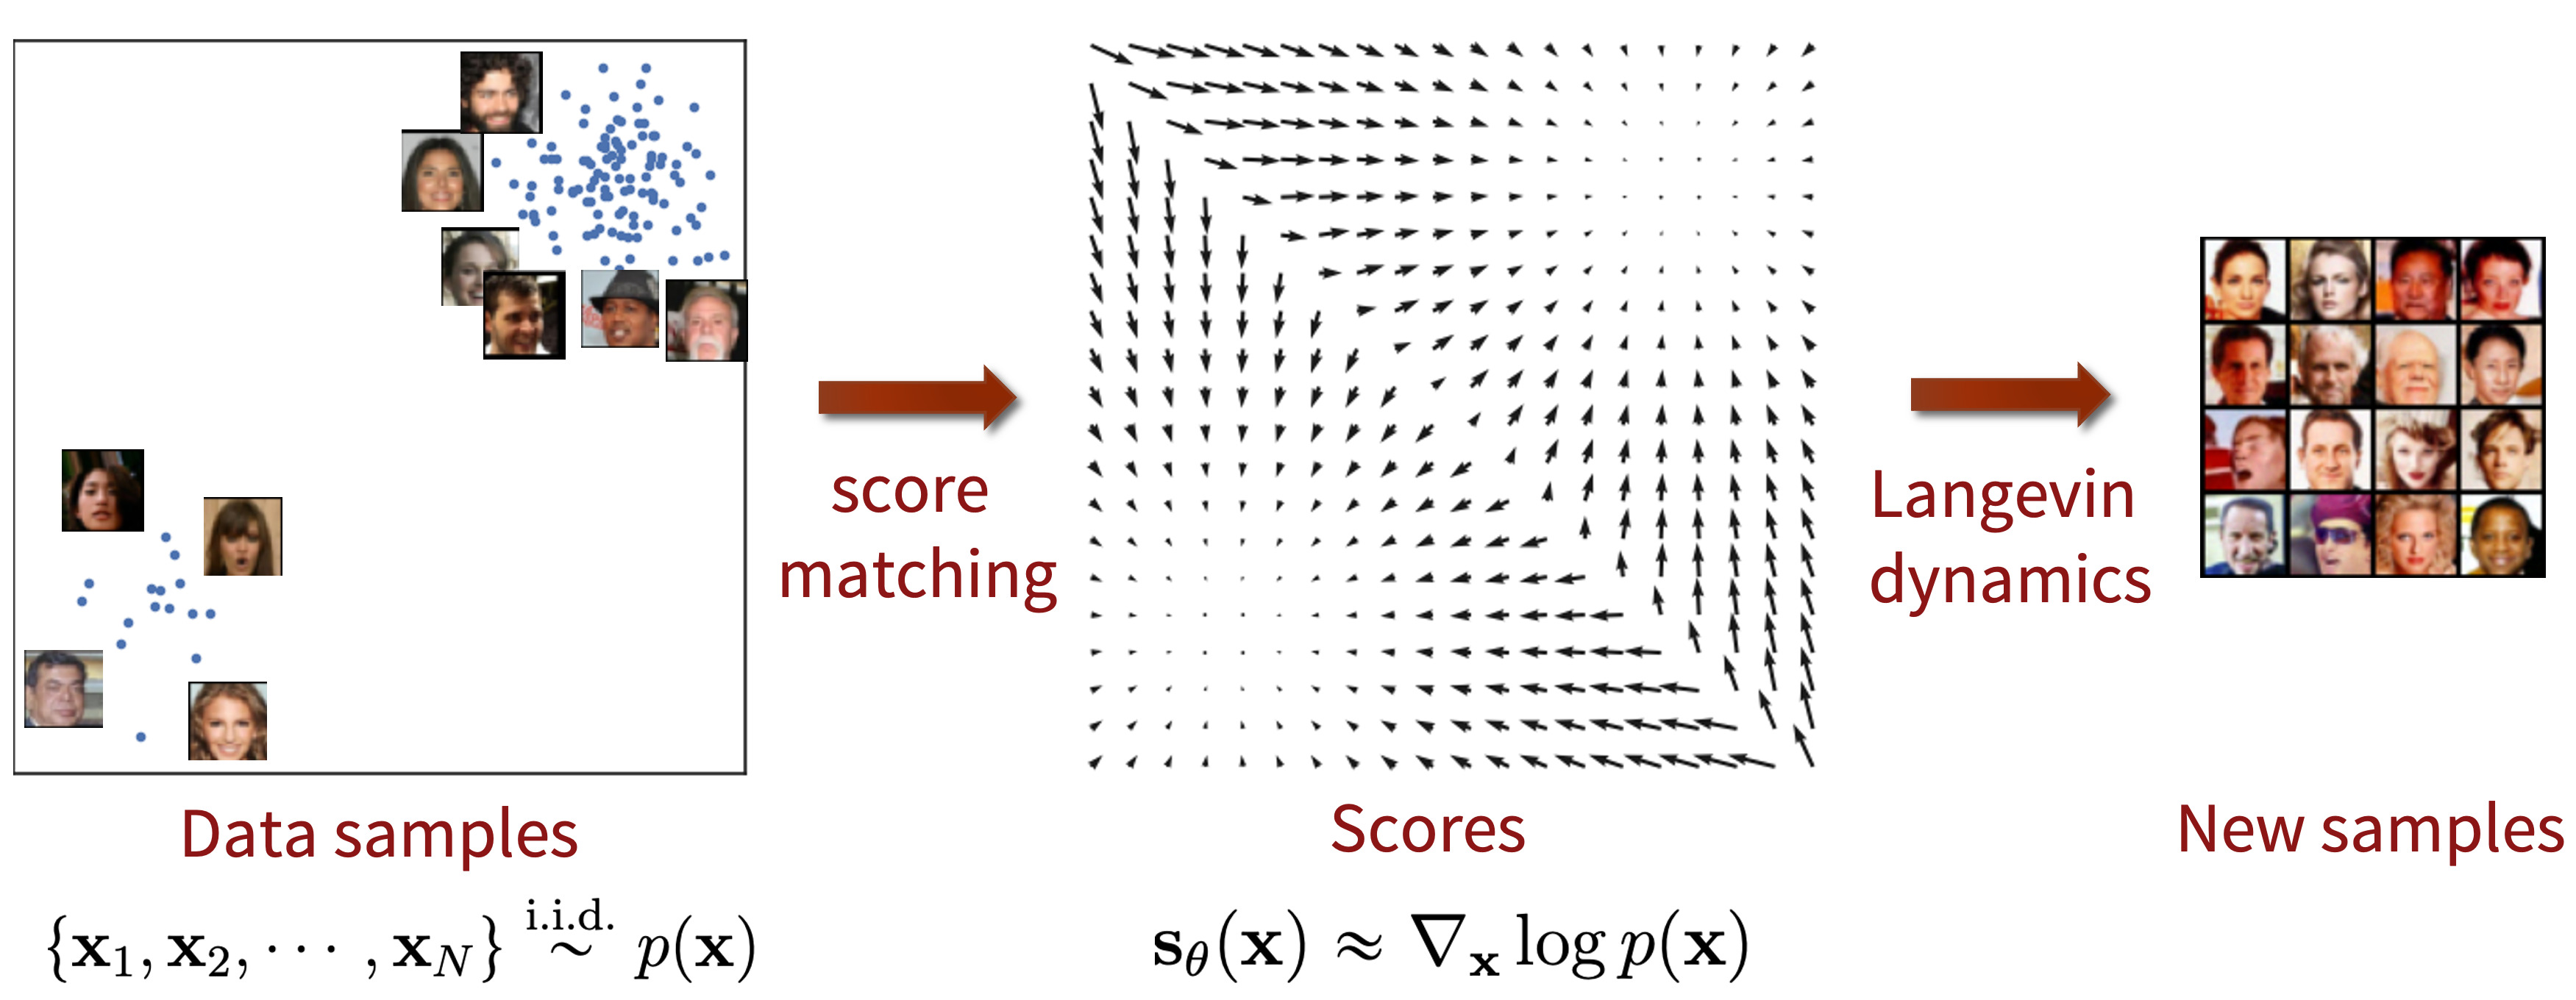
\includegraphics[width=0.8\linewidth]{figs/smld}
	\end{figure}
\end{frame}
%=======
\begin{frame}{Recap of Previous Lecture}
    \myfootnotewithlink{http://www.iro.umontreal.ca/~vincentp/Publications/smdae_techreport.pdf}{Vincent P. A Connection Between Score Matching and Denoising Autoencoders, 2010}

    Let us perturb the original data with Gaussian noise $q(\bx_{\sigma} | \bx) = \cN(\bx, \sigma^2 \cdot \bI)$.
    \vspace{-0.3cm}
    \[
        q(\bx_{\sigma}) = \int q(\bx_{\sigma} | \bx) \pd(\bx) d\bx.
    \]
    \vspace{-0.6cm} \\
    Then the solution of 
    \vspace{-0.2cm}
    \[
        \frac{1}{2} \bbE_{q(\bx_{\sigma})}\bigl\| \bs_{\btheta, \sigma}(\bx_{\sigma}) - \nabla_{\bx_{\sigma}} \log q(\bx_{\sigma}) \bigr\|^2_2 \rightarrow \min_{\btheta}
    \]
    \vspace{-0.5cm} \\
    satisfies $\bs_{\btheta, \sigma}(\bx_{\sigma}) \approx \bs_{\btheta, 0}(\bx_0) = \bs_{\btheta}(\bx)$ if $\sigma$ is sufficiently small.
    \begin{block}{Theorem (Denoising Score Matching)}
        \vspace{-0.8cm}
        \begin{multline*}
            \bbE_{q(\bx_{\sigma})}\bigl\| \bs_{\btheta, \sigma}(\bx_{\sigma}) - \nabla_{\bx_{\sigma}} \log q(\bx_{\sigma}) \bigr\|^2_2 = \\ = \bbE_{\pd(\bx)} \bbE_{q(\bx_{\sigma} | \bx)}\bigl\| \bs_{\btheta, \sigma}(\bx_{\sigma}) - \nabla_{\bx_{\sigma}} \log q(\bx_{\sigma} | \bx) \bigr\|^2_2 + \text{const}(\btheta)
        \end{multline*}
        \vspace{-0.7cm}
    \end{block}
    Here, $\nabla_{\bx_{\sigma}} \log q(\bx_{\sigma} | \bx) = - \frac{\bx_{\sigma} - \bx}{\sigma^2} = - \frac{\bepsilon}{\sigma}$. $\bs_{\btheta, \sigma}(\bx_{\sigma})$ attempts to \textbf{denoise} a corrupted sample.
\end{frame}
%=======
\begin{frame}{Recap of Previous Lecture}
    \myfootnotewithlink{https://yang-song.github.io/blog/2021/score/}{Song Y. Generative Modeling by Estimating Gradients of the Data Distribution, blog post, 2021}
	\vspace{-0.5cm}
	\[
		\bbE_{\pd(\bx)} \bbE_{\cN(0, \bI)}\left\| \bs_{\btheta, \sigma}(\bx + \sigma \bepsilon) + \frac{\bepsilon}{\sigma} \right\|_2^2 \rightarrow \min_{\btheta}
	\]
	\begin{minipage}{0.5\linewidth}
		\[
			\bx_{l + 1} = \bx_l + \frac{\eta}{2} \cdot \bs_{\btheta, \sigma}(\bx_l) + \sqrt{\eta} \cdot \bepsilon_l
		\]
		\vspace{-0.3cm}
		\begin{itemize}
			\item For \textbf{small} $\sigma$, $\bs_{\btheta, \sigma}(\bx)$ becomes inaccurate and Langevin dynamics fails to traverse modes
			\item For \textbf{large} $\sigma$, robustness in low-density regions is achieved, but the model learns a distribution that is overly corrupted
		\end{itemize}
	\end{minipage}%
	\begin{minipage}{0.5\linewidth}
		\begin{figure}
			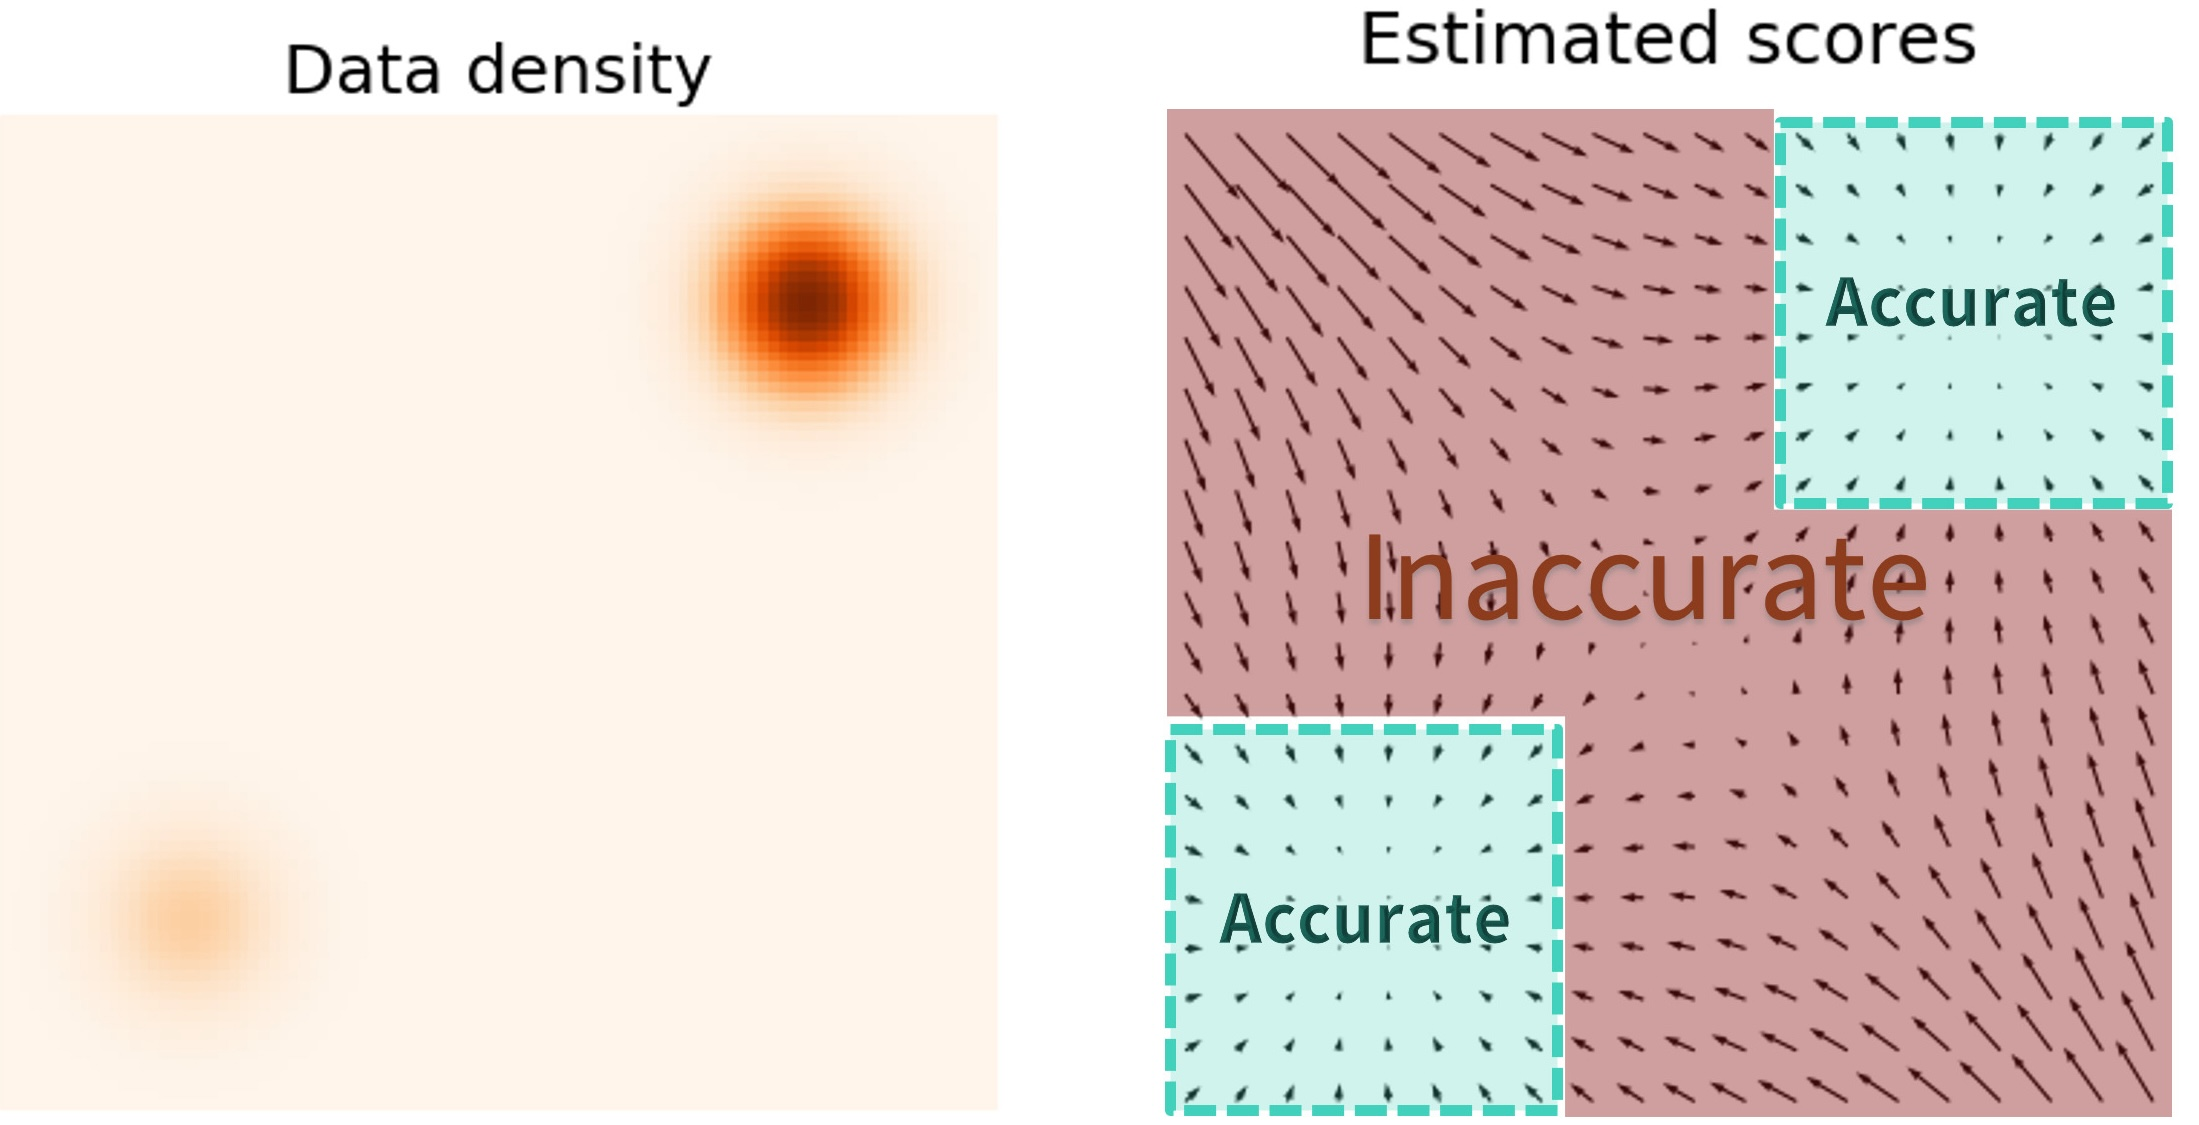
\includegraphics[width=\linewidth]{figs/pitfalls}
		\end{figure}
		\vspace{-0.3cm}
		\begin{figure}
			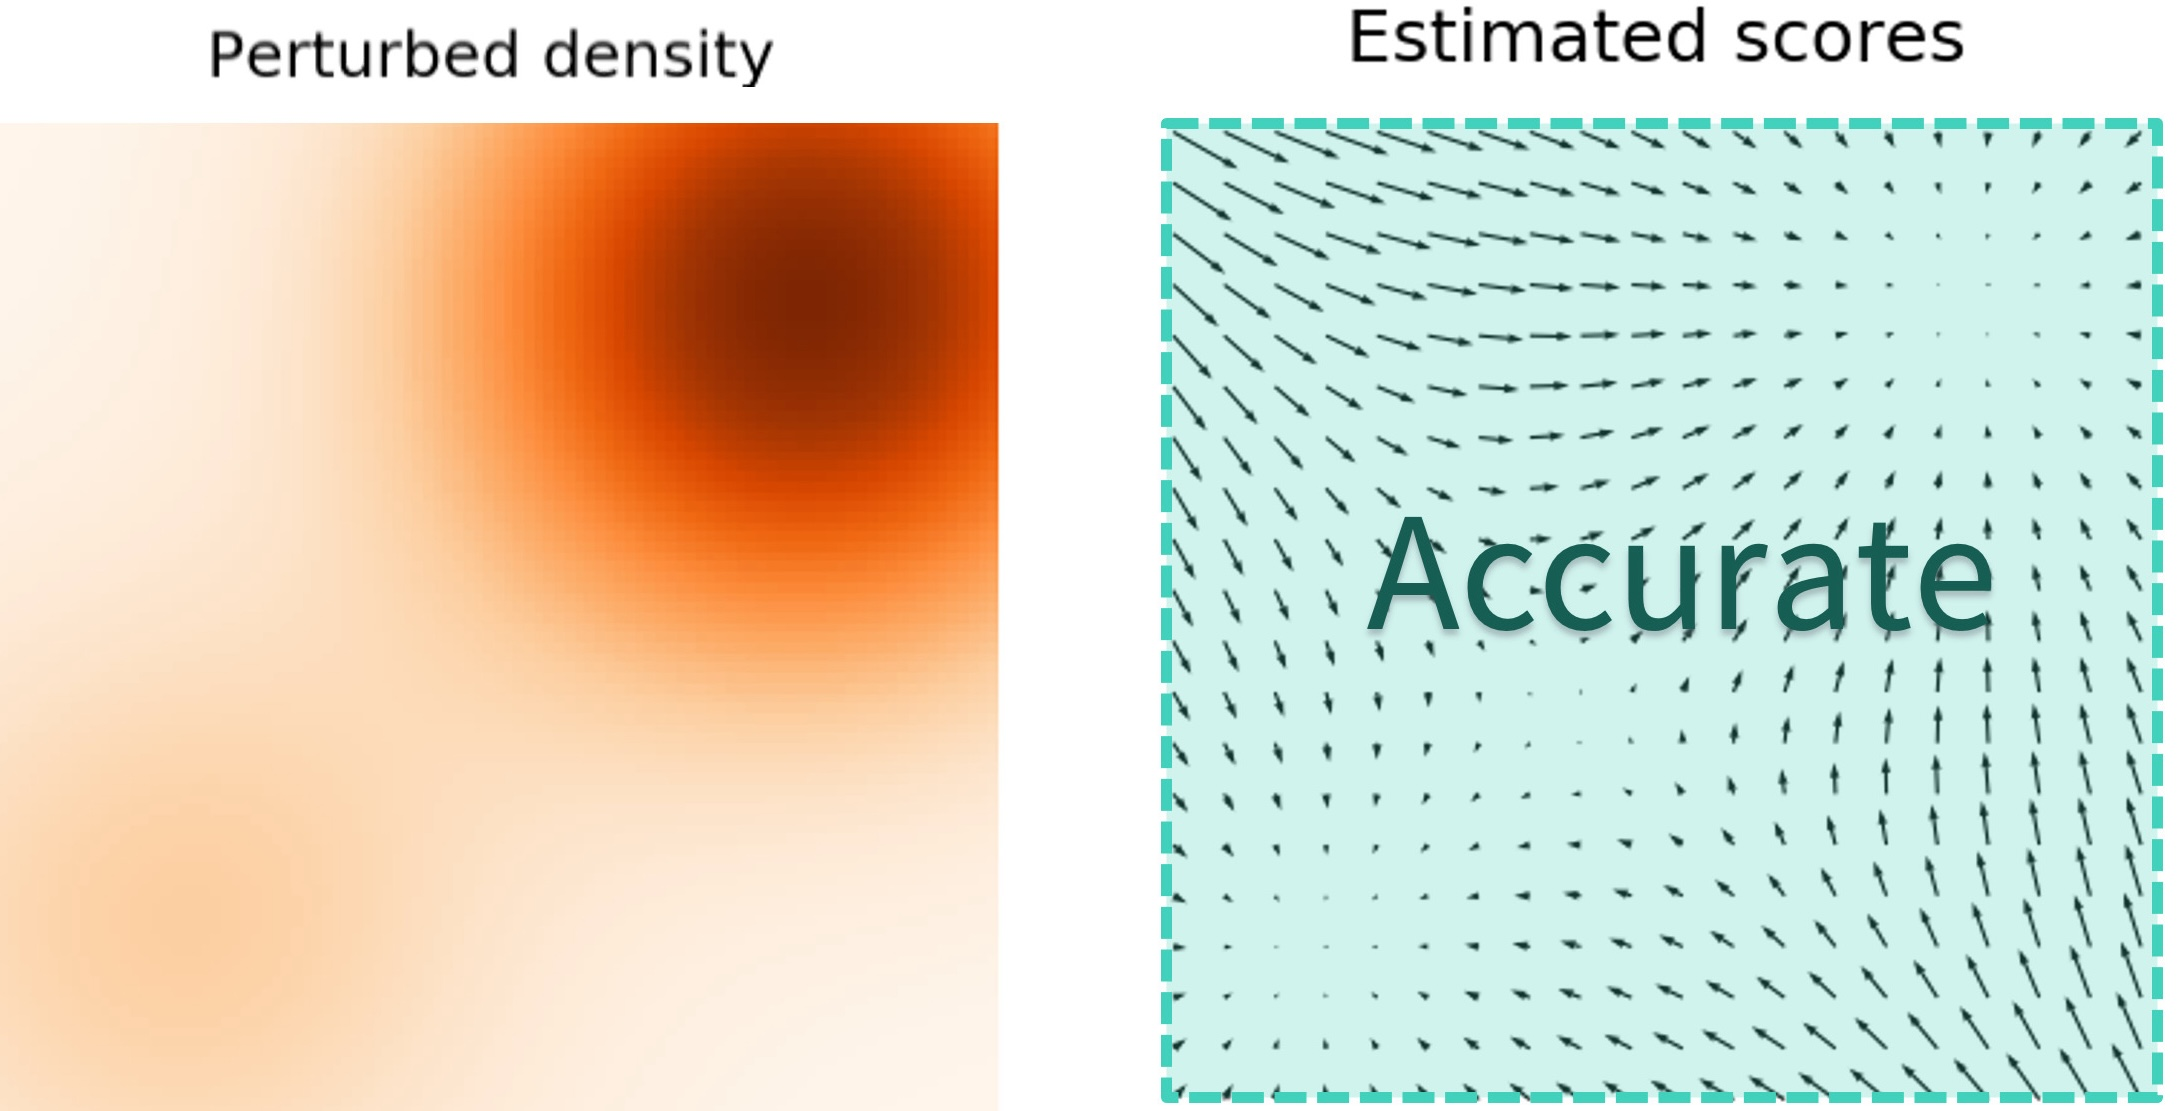
\includegraphics[width=\linewidth]{figs/single_noise}
		\end{figure}
	\end{minipage}
\end{frame}
%=======
\begin{frame}{Recap of Previous Lecture}
    \myfootnotewithlink{https://arxiv.org/abs/1907.05600}{Song Y. et al. Generative Modeling by Estimating Gradients of the Data Distribution, 2019}
    \begin{block}{Noise-Conditioned Score Network}
        \begin{itemize}
            \item Define a sequence of noise levels: $\sigma_1 < \sigma_2 < \dots < \sigma_T$.
            \item Train the denoising score function $\bs_{\btheta, \sigma_t}(\bx_t)$ for each noise level:
            \vspace{-0.3cm}
            \[
                \sum_{t=1}^T {\color{violet}\sigma_t^2} \cdot \bbE_{\pd(\bx)} \bbE_{q(\bx_t | \bx)}\bigl\| \bs_{\btheta, \sigma_t}(\bx_t) - \nabla_{\bx_t} \log q(\bx_t | \bx) \bigr\|^2_2 \rightarrow \min_{\btheta}
            \]
            \vspace{-0.5cm}
            \item Sample using \textbf{annealed} Langevin dynamics (for $t=1, \dots, T$).
        \end{itemize}
    \end{block}
    \vspace{-0.3cm}
    \begin{figure}
        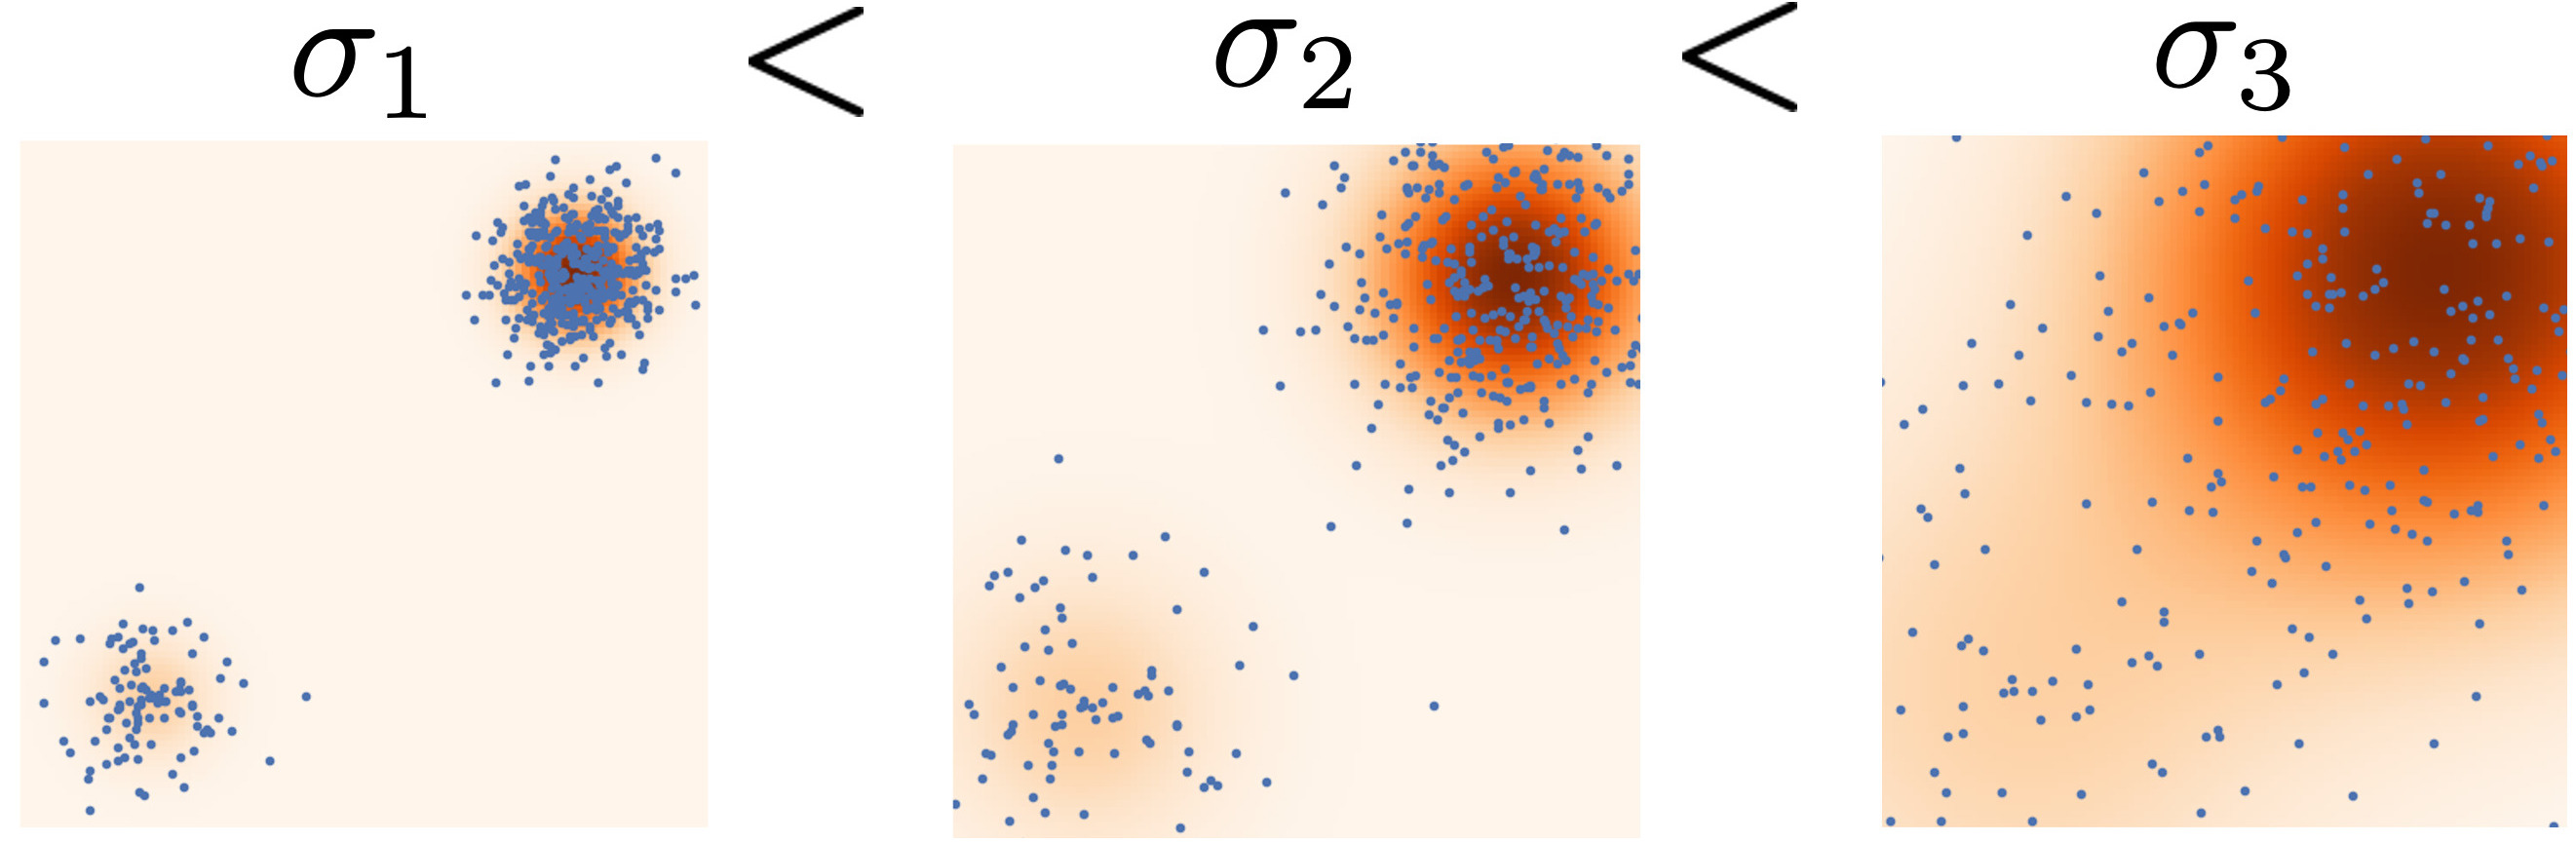
\includegraphics[width=0.55\linewidth]{figs/multi_scale}
    \end{figure}
    \vspace{-0.3cm}
    \begin{figure}
        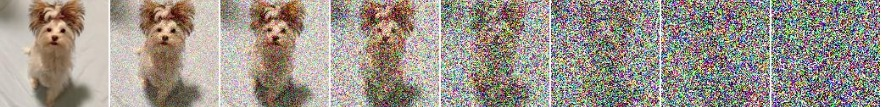
\includegraphics[width=\linewidth]{figs/duoduo}
    \end{figure}
\end{frame}
%=======
\begin{frame}{Recap of Previous Lecture}
    \myfootnotewithlink{https://arxiv.org/abs/2006.09011}{Song Y. et al. Improved Techniques for Training Score-Based Generative Models, 2020}
    \begin{block}{NCSN Training}
        \begin{enumerate}
            \item Obtain a sample $\bx_0 \sim \pd(\bx)$.
            \item Sample noise level $t \sim U\{1, T\}$ and noise $\bepsilon \sim \cN(0, \bI)$.
            \item Construct noisy image $\bx_t = \bx_0 + \sigma_t \cdot \bepsilon$.
            \item Compute the loss $ \cL = \sigma_t^2 \cdot \| \bs_{\btheta, \sigma_t}(\bx_t) + \frac{\bepsilon}{\sigma_t} \|^2 $.
        \end{enumerate}
    \end{block}
    \begin{block}{NCSN Sampling (Annealed Langevin Dynamics)}
        \begin{itemize}
            \item Sample $\bx_0 \sim \cN(0, \sigma_T^2 \cdot \bI) \approx q(\bx_T)$.
            \item Apply $L$ steps of Langevin dynamics:
            \vspace{-0.2cm}
            \[
                \bx_l = \bx_{l-1} + \frac{\eta_t}{2} \cdot \bs_{\btheta, \sigma_t}(\bx_{l - 1}) + \sqrt{\eta_t} \cdot \bepsilon_l.
            \] 
            \vspace{-0.5cm}
            \item Update $\bx_0 := \bx_L$ and proceed to the next $\sigma_t$.
        \end{itemize}
    \end{block}
\end{frame}
%=======
\begin{frame}{Outline}
	\tableofcontents
\end{frame}
%=======
\section{Forward Gaussian Diffusion Process}
%=======
\begin{frame}{Generative Models Taxonomy}
	\renderTaxonomy{ddpm}
\end{frame}
%=======
\begin{frame}{Forward Gaussian Diffusion Process}
    \myfootnotewithlink{http://proceedings.mlr.press/v37/sohl-dickstein15.pdf}{Sohl-Dickstein J. Deep Unsupervised Learning using Nonequilibrium Thermodynamics, 2015}

	Let $\bx_0 = \bx \sim \pd(\bx)$, $\beta_t \ll 1$. Define a Markov chain:
	\[
		\bx_t = \sqrt{1 - \beta_t} \bx_{t-1} + \sqrt{\beta_t} \bepsilon_t, \;\; \bepsilon_t \sim \cN(0, \bI)
	\]
	\vspace{-0.5cm}
    \eqpause
	\[
		q(\bx_t | \bx_{t-1}) = \cN(\sqrt{1 - \beta_t} \bx_{t-1}, \beta_t \bI)
	\]
    \eqpause
	\vspace{-0.5cm}
	\begin{block}{Langevin Dynamics}
		\vspace{-0.3cm}
		\[
			\bx_{l + 1} = \bx_l + \frac{ \color{violet} \eta}{2} \cdot {\color{teal}\nabla_{\bx_l} \log \pt(\bx_l)} + \sqrt{ \color{violet} \eta} \bepsilon_l, \quad \bepsilon_l \sim \cN(0, \bI)
		\]
		\vspace{-0.5cm}
	\end{block}
    \eqpause
	\vspace{-0.7cm}
	\begin{multline*}
		\bx_t = \sqrt{1 - \beta_t}\, \bx_{t - 1} + \sqrt{\beta_t} \bepsilon_t \approx \left(1 - \frac{\beta_t}{2}\right)\bx_{t-1} + \sqrt{\beta_t} \bepsilon_t = \\
		= \bx_{t-1} + \frac{ \color{violet}  \beta_t}{2} {\color{teal} ( -\bx_{t-1} )} + \sqrt{ \color{violet}  \beta_t} \bepsilon_t
	\end{multline*}
    \eqpause
	\vspace{-0.7cm}
	\begin{itemize}
		\item ${\color{violet} \beta_t = \eta }$
		\item ${\color{teal} \nabla_{\bx_{t-1}}\log p(\bx_{t-1} | \btheta) = - \bx_{t-1} = \nabla_{\bx_{t-1}} \log \cN(0, \bI)}$
	\end{itemize}
 \end{frame}
%=======
\begin{frame}{Forward Gaussian Diffusion Process}
    \myfootnotewithlink{http://proceedings.mlr.press/v37/sohl-dickstein15.pdf}{Sohl-Dickstein J. Deep Unsupervised Learning using Nonequilibrium Thermodynamics, 2015}
	\[
		\bx_t = \sqrt{1 - \beta_t} \bx_{t-1} + \sqrt{\beta_t} \bepsilon_t, \;\; \bepsilon_t \sim \cN(0, \bI)
	\]
	\[
		q(\bx_t | \bx_{t-1}) = \cN(\sqrt{1 - \beta_t} \bx_{t-1}, \beta_t \bI)
	\]
    \eqpause
	\vspace{-0.5cm}
	\begin{block}{Statement 1}
		Let $\alpha_t = 1 - \beta_t$ and $\bar{\alpha}_t = \prod_{s=1}^t \alpha_s = \prod_{s=1}^t (1 - \beta_s)$. Then
		\[
			q(\bx_t | \bx_0) = \cN(\sqrt{\bar{\alpha}_t} \,\bx_0, (1 - \bar{\alpha}_t) \bI)
		\]
        \eqpause
		Thus, samples at any timestep $t$ can be generated directly from $\bx_0$
		\vspace{-0.2cm}
		{\small
		\begin{multline*}
			\bx_t = \sqrt{\alpha_t} {\color{teal}\bx_{t-1}} + \sqrt{1 - \alpha_t} \bepsilon_t
			\nextonslide{ = \\ = \sqrt{\alpha_t} ( {\color{teal} \sqrt{\alpha_{t-1}} \bx_{t-2} + \sqrt{1 - \alpha_{t-1}} \bepsilon_{t-1} } ) + \sqrt{1 - \alpha_t} \bepsilon_t}
			\nextonslide{ = \\ = \sqrt{\alpha_t \alpha_{t-1}} \bx_{t-2} + ( {\color{violet} \sqrt{\alpha_t (1-\alpha_{t-1})} \bepsilon_{t-1} + \sqrt{1-\alpha_t} \bepsilon_t } )}
			\nextonslide{ = \\ = \sqrt{\alpha_t \alpha_{t-1}} \bx_{t-2} + {\color{violet} \sqrt{1-\alpha_t \alpha_{t-1}} \bepsilon'_t}}
			\nextonslide{= \\ = \ldots = \sqrt{\bar{\alpha}_t}\, \bx_0 + \sqrt{1-\bar{\alpha}_t} \bepsilon, \quad \bepsilon \sim \cN(0, \bI)}
		\end{multline*}
		}
	\end{block}
 \end{frame}
%=======
\begin{frame}{Forward Gaussian Diffusion Process}
    \myfootnotewithlink{https://arxiv.org/abs/2403.18103}{Chan S. Tutorial on Diffusion Models for Imaging and Vision, 2024}
	\vspace{-0.3cm}
	{\small
	\[
		q(\bx_t | \bx_{t-1}) = \cN\left(\sqrt{1 - \beta_t} \bx_{t-1}, \beta_t \bI\right); \quad q(\bx_t | \bx_0) = \cN\left(\sqrt{\bar{\alpha}_t} \bx_0, (1 - \bar{\alpha}_t) \bI\right)
	\]
	}
	\vspace{-0.7cm}
	\begin{figure}
		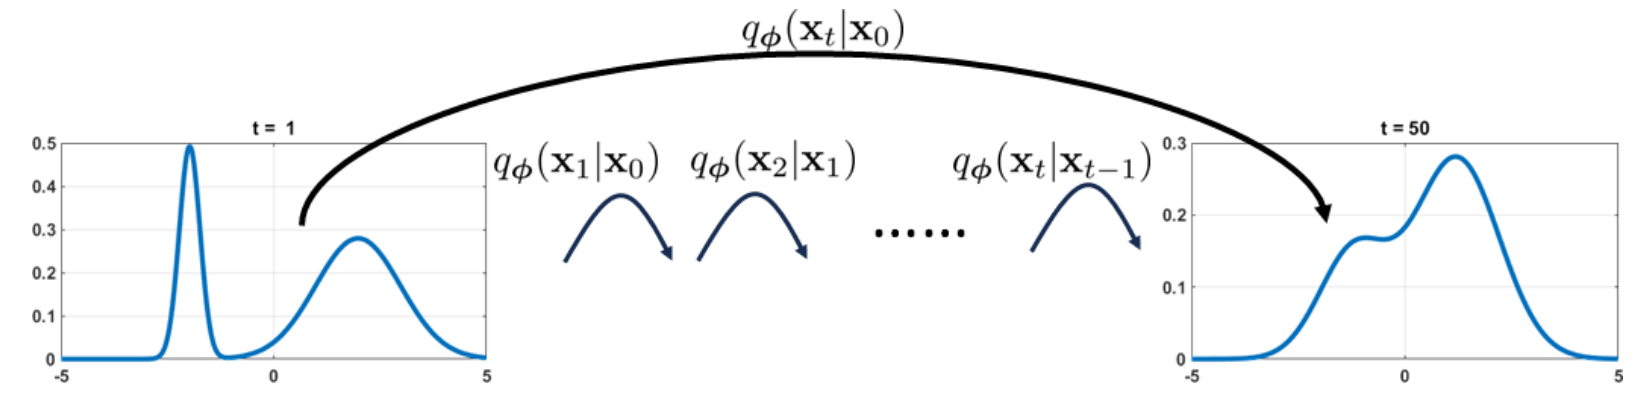
\includegraphics[width=0.8\linewidth]{figs/conditional_diffusion}
	\end{figure}
    \eqpause
	\vspace{-0.3cm}
	\begin{block}{Statement 2}
		Applying the Markov chain to any distribution $\pd(\bx)$ yields $\bx_\infty \sim p_\infty(\bx) = \cN(0, \bI)$, the \textbf{stationary} (limiting) distribution:
		\[
			p_\infty(\bx) = \int q(\bx | \bx') p_\infty(\bx') d\bx' 
		\]

		\vspace{-0.7cm}
        \eqpause
		\[
			p_\infty(\bx) = \int q(\bx_\infty | \bx_0) \pd(\bx_0) d\bx_0 \approx \cN(0, \bI) \int \pd(\bx_0) d\bx_0 = \cN(0, \bI)
		\]
	\end{block}
	\eqpause
	\vspace{-0.3cm}
	\textbf{Note:} This holds iff $\bar{\alpha}_t \rightarrow 0$, i.e., $\sum_{t=1}^{\infty} \beta_t = +\infty$.
 \end{frame}
%=======
\begin{frame}{Forward Gaussian Diffusion Process}
    \myfootnotewithlink{https://ayandas.me/blog-tut/2021/12/04/diffusion-prob-models.html}{Das A. An introduction to Diffusion Probabilistic Models, blog post, 2021}
	\textbf{Diffusion} describes the migration of particles from regions of high density to those of low density.
	\vspace{-0.2cm}
	\begin{figure}
		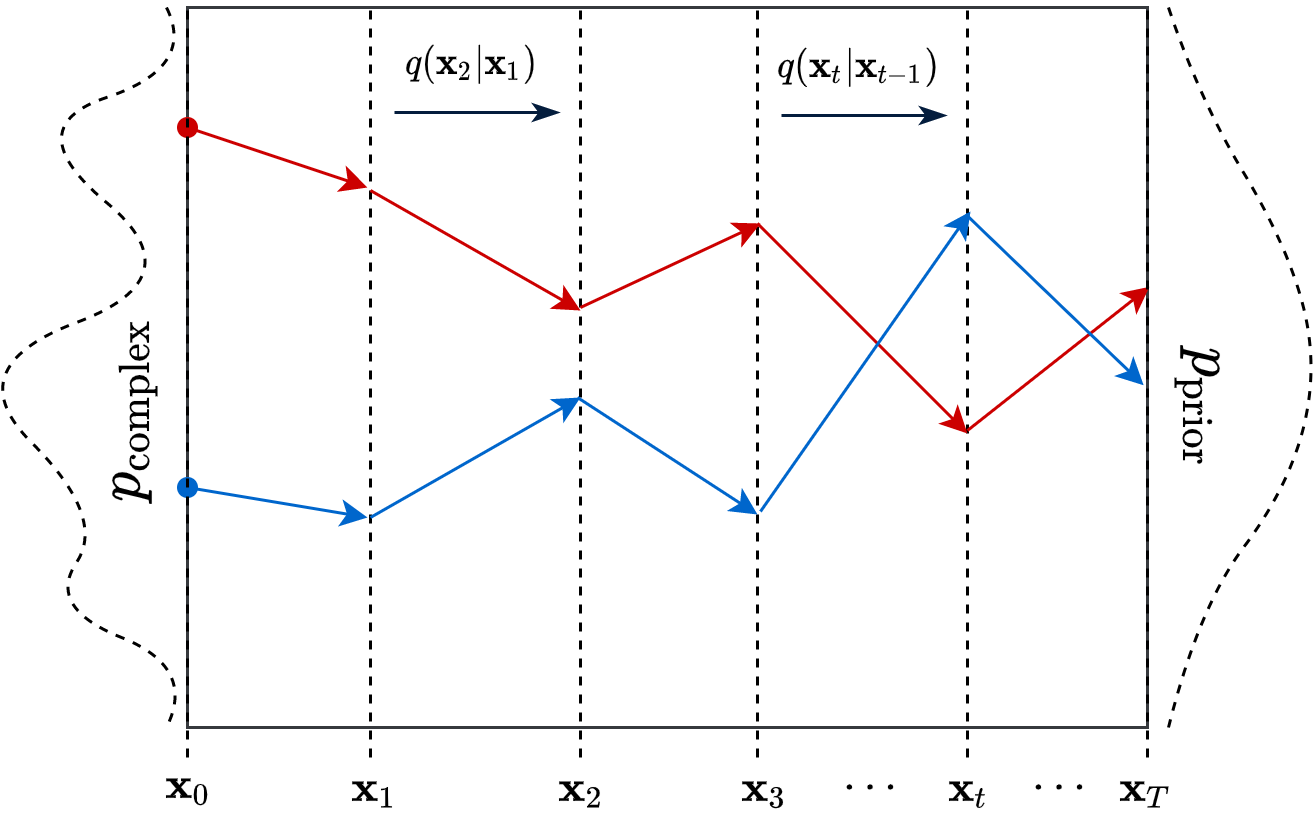
\includegraphics[width=0.5\linewidth]{figs/diffusion_over_time}
	\end{figure}
    \eqpause
	\vspace{-0.5cm}
	\begin{enumerate}
		\item $\bx_0 = \bx \sim \pd(\bx)$
		\item $\bx_t = \sqrt{1 - \beta_t} \bx_{t-1} + \sqrt{\beta_t} \bepsilon$, $\bepsilon \sim \cN(0, \bI)$, $t \geq 1$
		\item After $T \gg 1$ steps: $\bx_T \sim p_\infty(\bx) = \cN(0, \bI)$
	\end{enumerate}
    \eqpause
	If this process can be reversed, we can sample from $\pd(\bx)$ by starting from noise $p_\infty(\bx) = \cN(0, \bI)$. \\
	Our goal now becomes inverting this diffusion.
\end{frame}
%=======
\begin{frame}{Denoising Score Matching}
	\begin{block}{NCSN} 
		\vspace{-0.7cm} 
		\[
			q(\bx_t | \bx_0) = \cN(\bx_0, \sigma_t^2 \bI), \quad q(\bx_1) \approx \pd(\bx), \quad q(\bx_T) \approx \cN(0, \sigma_T^2 \bI)
		\]
		\[
			\nabla_{\bx_t} \log q(\bx_t | \bx) = - \frac{\bx_t - \bx}{\sigma_t^2}
		\]
		\vspace{-0.6cm} 
	\end{block}
    \eqpause
	\begin{block}{Gaussian Diffusion}
		\vspace{-0.7cm} 
		\[
			q(\bx_t | \bx_0) = \cN(\sqrt{\bar{\alpha}_t} \bx_0, (1 - \bar{\alpha}_t) \bI), \quad q(\bx_1) \approx \pd(\bx), \quad q(\bx_T) \approx \cN(0, \bI)
		\]
		\[
			\nabla_{\bx_t} \log q(\bx_t | \bx_0) = - \frac{\bx_t - \sqrt{\bar{\alpha}_t} \bx_0}{1 - \bar{\alpha}_t}
		\]
		\vspace{-0.6cm} 
	\end{block}
    \eqpause
	\begin{block}{Theorem (Denoising Score Matching)}
		\vspace{-0.7cm}
		\begin{multline*}
			\bbE_{q(\bx_t)}\left\| \bs_{\btheta, t}(\bx_t) - \nabla_{\bx_t} \log q(\bx_t) \right\|_2^2 = \\
			= \bbE_{\pd(\bx)} \bbE_{q(\bx_t | \bx)}\left\| \bs_{\btheta, t}(\bx_t) - \nabla_{\bx_t} \log q(\bx_t | \bx) \right\|_2^2 + \text{const}(\btheta)
		\end{multline*}
		\vspace{-0.5cm}
	\end{block}
    \eqpause
	\textbf{Note:} This enables applying the NCSN approach with annealed Langevin dynamics to diffusion-based denoising models.
\end{frame}
%=======
\section{Reverse Gaussian Diffusion Process}
%=======
\begin{frame}{Reverse Gaussian Diffusion Process}
    \myfootnotewithlink{https://lilianweng.github.io/posts/2021-07-11-diffusion-models/}{Weng L. What are Diffusion Models?, blog post, 2021}
	\begin{figure}
		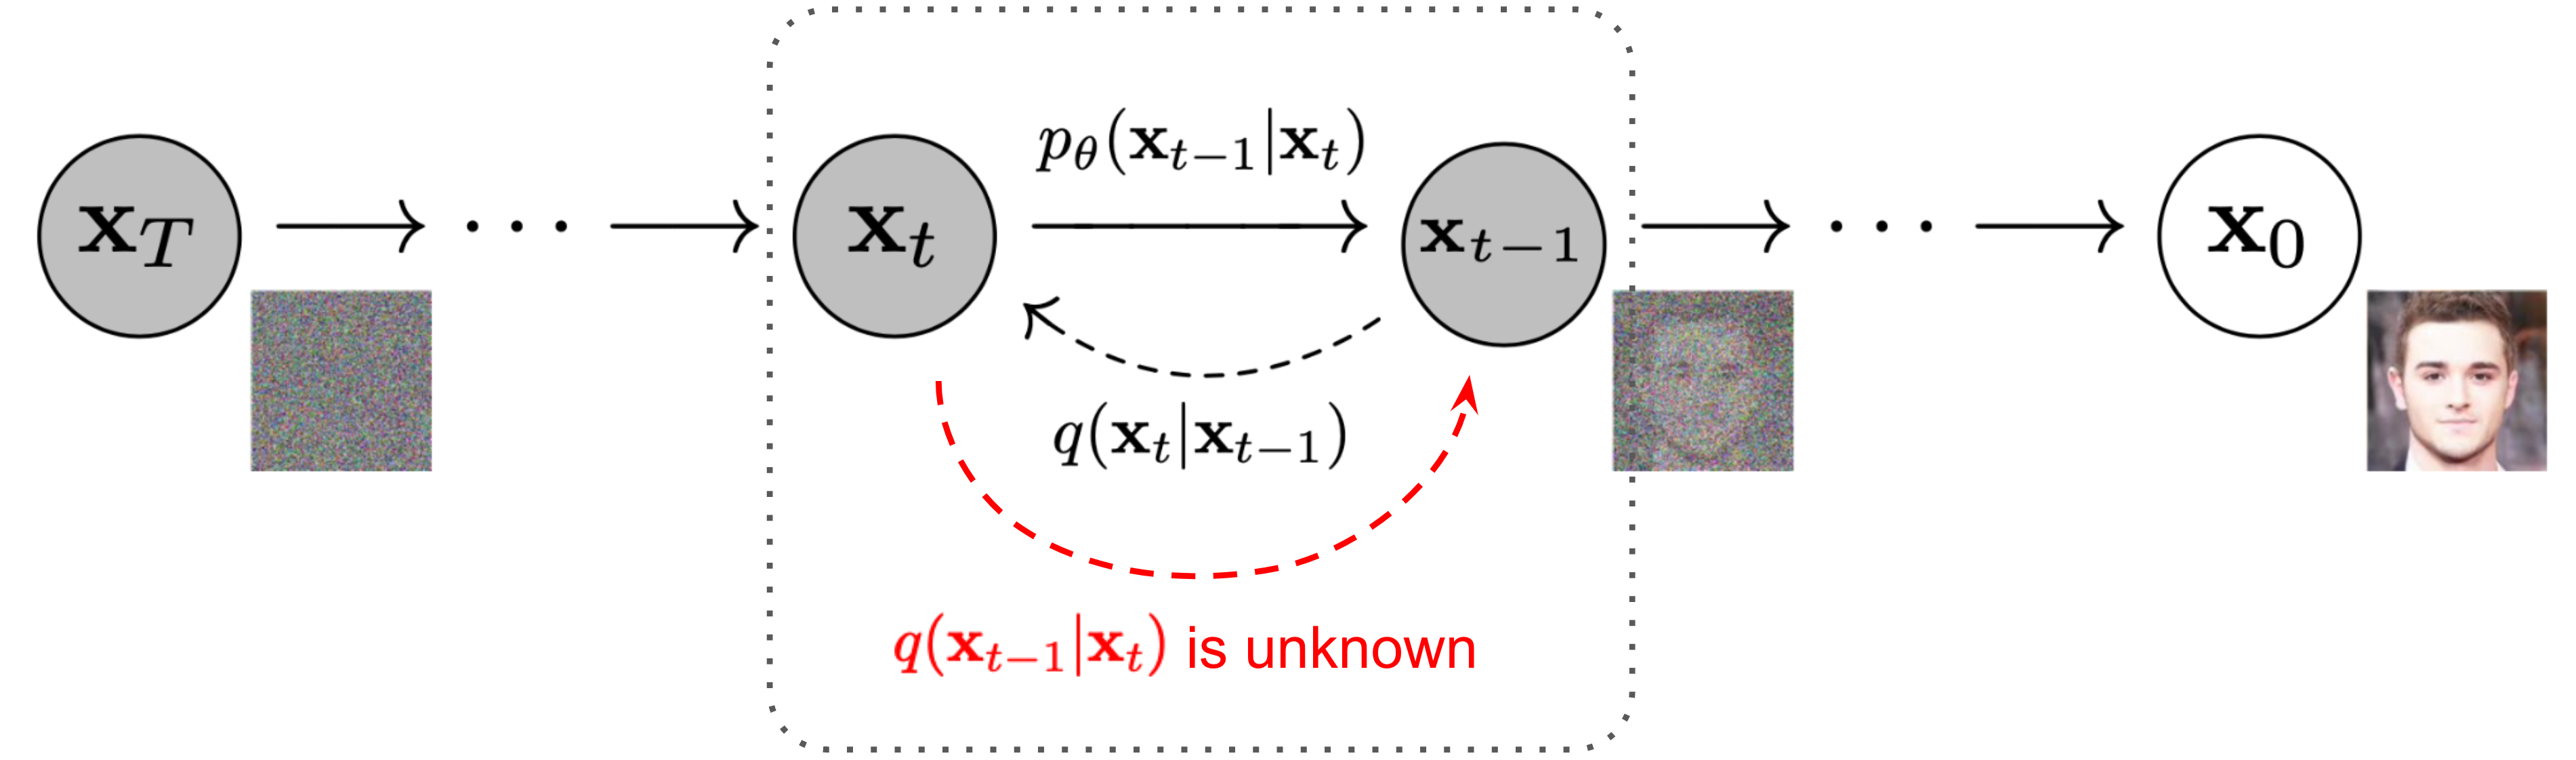
\includegraphics[width=0.8\linewidth]{figs/DDPM}
	\end{figure}
    \eqpause
	\vspace{-0.5cm}
	\begin{block}{Forward Process}
		\vspace{-0.3cm}
		\[
			q(\bx_t | \bx_{t-1}) = \cN\left(\sqrt{1 - \beta_t} \bx_{t-1}, \beta_t \bI\right)
		\]
		\vspace{-0.5cm}
	\end{block}
    \eqpause
	\begin{block}{Reverse Process}
		\vspace{-0.3cm}
		\[
			q(\bx_{t-1}| \bx_{t}) = \frac{q(\bx_{t}| \bx_{t-1}) {\color{violet}q(\bx_{t-1})}}{{\color{violet}q(\bx_{t})}} 
			\approx \pt(\bx_{t - 1} | \bx_t)
		\]
        \eqpause
		\vspace{-0.3cm}
		${\color{violet}q(\bx_{t-1})}$ and ${\color{violet}q(\bx_{t})}$ are intractable:
		\[
			q(\bx_{t}) = \int q(\bx_{t} | \bx_0) \pd(\bx_0) d\bx_0
		\]
	\end{block}
\end{frame}
%=======
\begin{frame}{Reverse Gaussian Diffusion Process}
    \myfootnote{\href{}{Feller W. On the theory of stochastic processes, with particular reference to applications, 1949} \\ 
    \href{https://arxiv.org/abs/2112.07804}{Xiao Z., Kreis K., Vahdat A. Tackling the generative learning trilemma with denoising diffusion GANs, 2021}}
	\vspace{-0.4cm}
	\[
		q(\bx_{t-1}|\bx_{t}) = \frac{q(\bx_{t}|\bx_{t-1}) {\color{violet}q(\bx_{t-1})}}{{\color{violet}q(\bx_{t})}} 
	\]
	\vspace{-0.4cm}
	\begin{block}{Theorem (Feller, 1949)}
		If $\beta_t$ is sufficiently small, $q(\bx_{t-1}|\bx_t)$ is Gaussian {\color{gray}(thus, diffusion requires $T \approx 1000$ steps for convergence)}
	\end{block}
	\eqpause
	\vspace{-0.3cm}
	\begin{figure}
		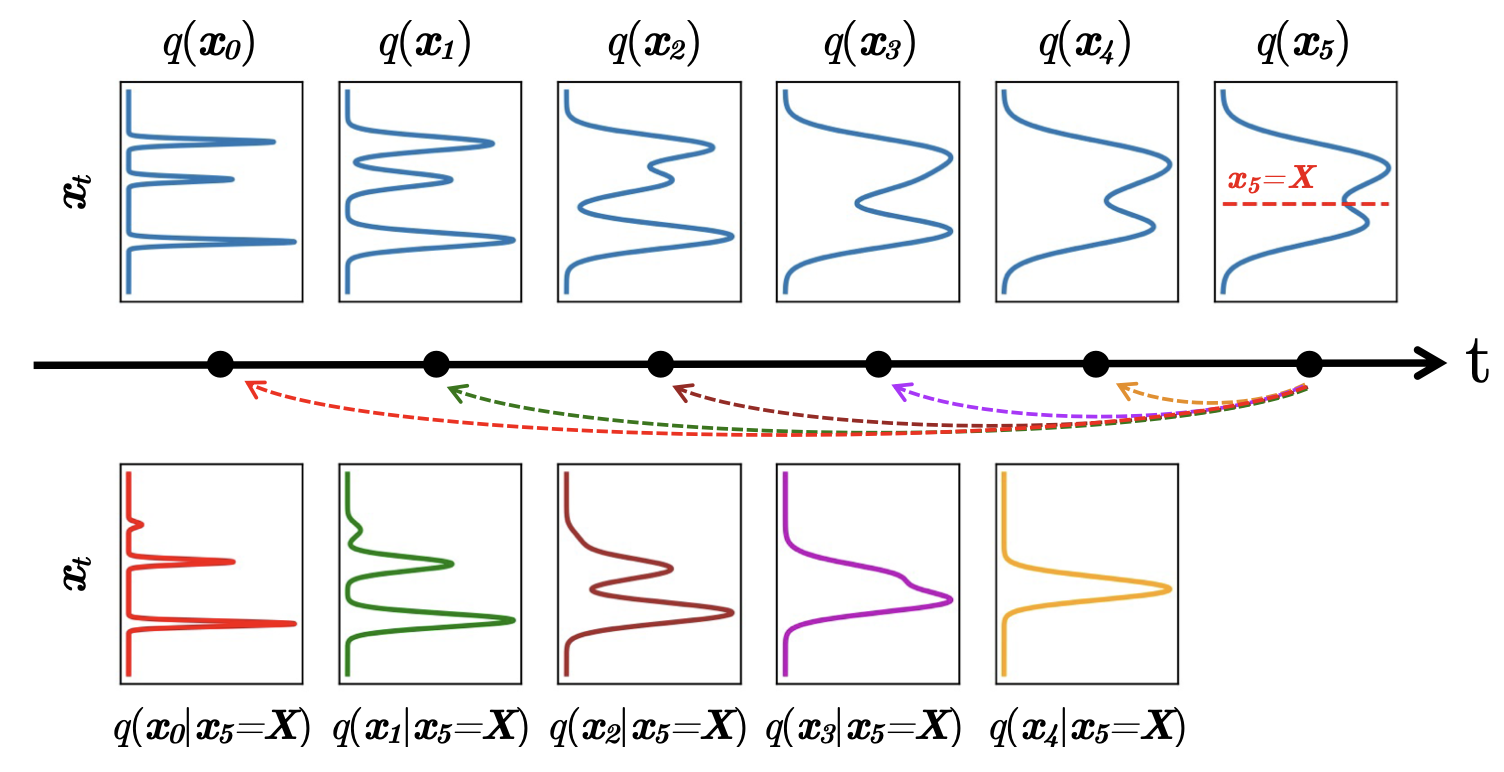
\includegraphics[width=0.7\linewidth]{figs/inverse_distr_1d}
	\end{figure}
\end{frame} 
%=======
\begin{frame}{Reverse Gaussian Diffusion Process (Ancestral Sampling)}
    \myfootnotewithlink{https://lilianweng.github.io/posts/2021-07-11-diffusion-models/}{Weng L. What are Diffusion Models?, blog post, 2021}
	\vspace{-0.3cm} 
	\begin{figure}
		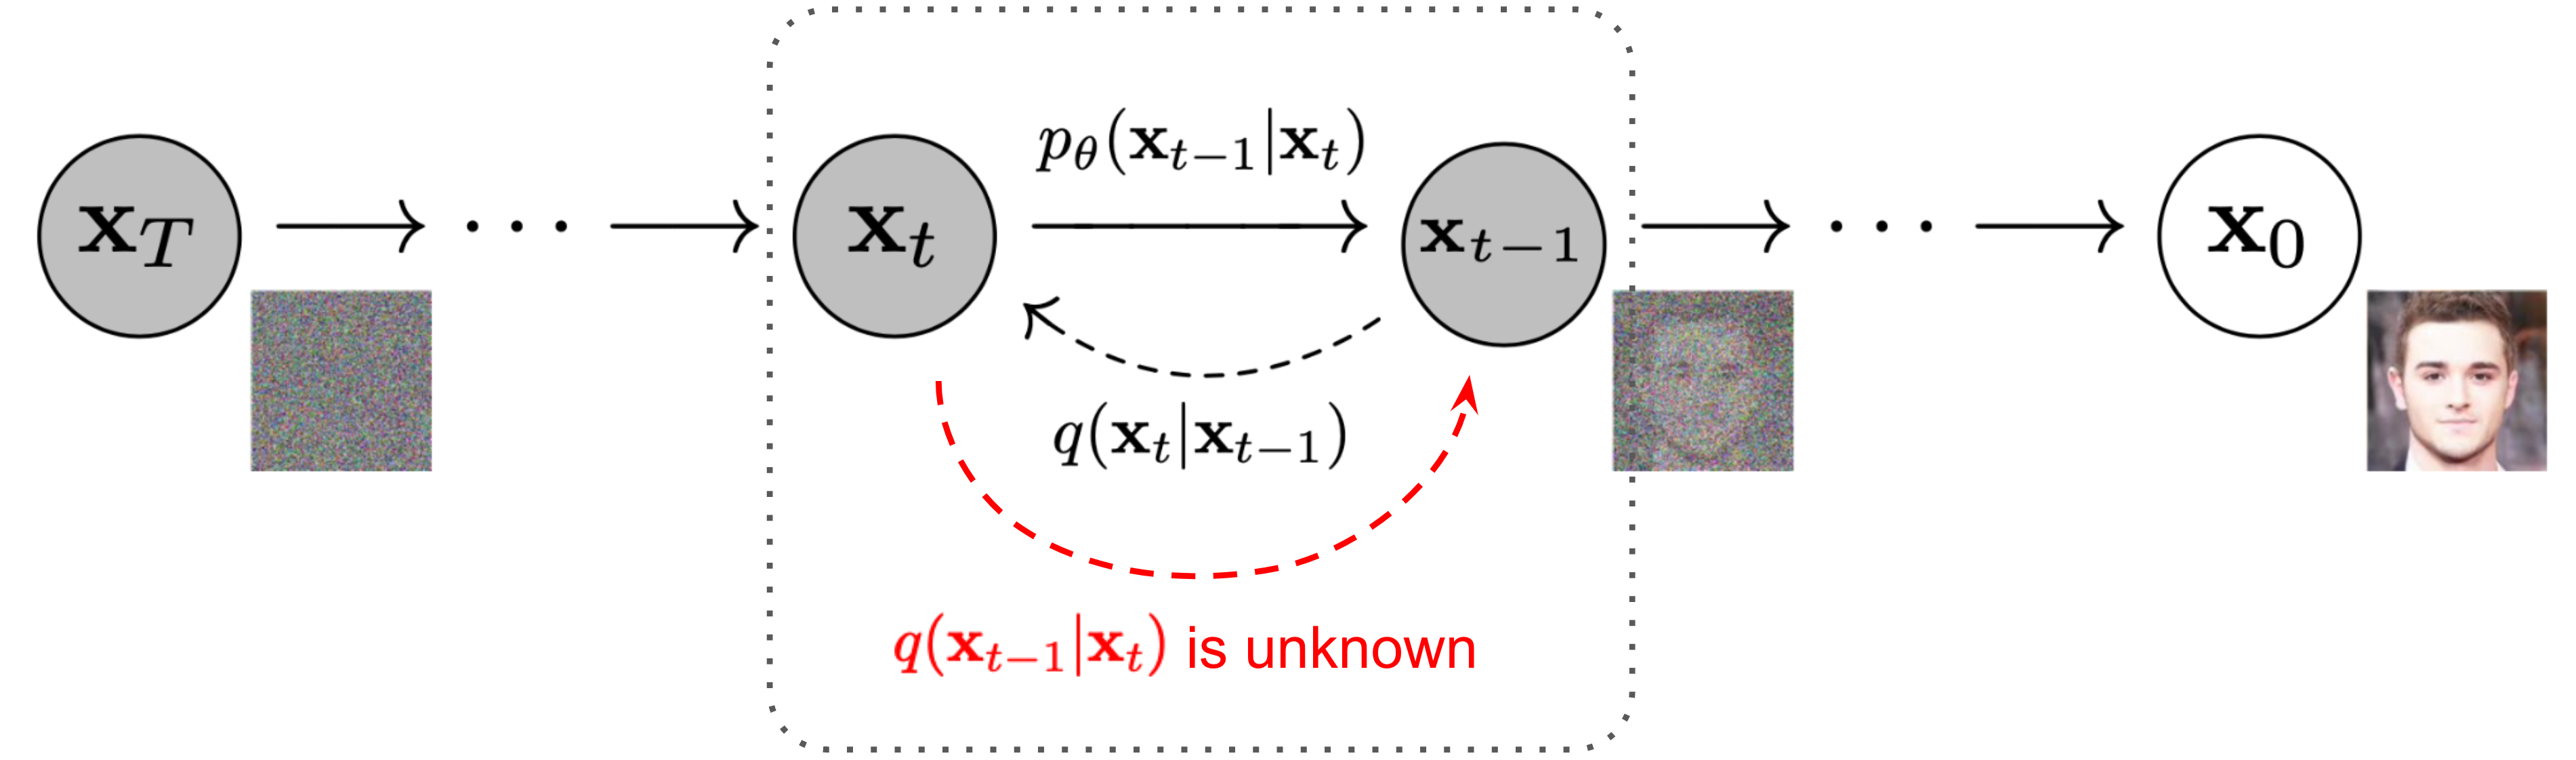
\includegraphics[width=0.8\linewidth]{figs/DDPM}
	\end{figure}
	\vspace{-0.3cm} 
	Define the reverse process as: 
	\vspace{-0.2cm}
	\[
		q(\bx_{t-1}|\bx_{t}) \approx \pt(\bx_{t - 1} | \bx_t) = \cN\bigl(\bmu_{\btheta, t}(\bx_t), \bsigma^2_{\btheta, t}(\bx_t)\bigr)
	\]
	{\color{gray}Feller's theorem justifies this Gaussian assumption.}
	\eqpause
	\begin{minipage}{0.5\linewidth}
		\begin{block}{Forward Process}
			\begin{enumerate}
				\item $\bx_0 = \bx \sim \pd(\bx)$
				\item $\bx_t = \sqrt{1 - \beta_t} \bx_{t-1} + \sqrt{\beta_t} \bepsilon$
				\item $\bx_T \sim p_\infty(\bx) = \cN(0, \bI)$
			\end{enumerate}
		\end{block}
	\end{minipage}%
    \eqpause
	\begin{minipage}{0.55\linewidth}
		\begin{block}{Reverse Process}
			\begin{enumerate}
				\item $\bx_T \sim p_\infty(\bx) = \cN(0, \bI)$
				\item $\bx_{t-1} = \bsigma_{\btheta, t}(\bx_t) \bepsilon + \bmu_{\btheta, t}(\bx_t)$
				\item $\bx_0 = \bx \sim \pd(\bx)$
			\end{enumerate}
		\end{block}
	\end{minipage}
    \eqpause
	\textbf{Note:} The forward process is non-learnable, i.e., it does not involve trainable parameters
\end{frame}
%=======
\begin{frame}{Conditioned Reverse Distribution}
    \myfootnotewithlink{https://arxiv.org/abs/2006.11239}{Ho J. Denoising Diffusion Probabilistic Models, 2020}
    \begin{block}{Reverse Kernel (\textbf{Intractable})}
        \vspace{-0.3cm}
        \[
            q(\bx_{t-1}|\bx_{t}) = \frac{q(\bx_{t}|\bx_{t-1}) {\color{violet}q(\bx_{t-1})}}{{\color{violet}q(\bx_{t})}} 
        \]
        \vspace{-0.5cm}
    \end{block}
    \eqpause
    \begin{block}{Conditioned Reverse Kernel (\textbf{Tractable})}
        \vspace{-0.6cm}
        \begin{align*}
            q(\bx_{t-1}|\bx_{t}, {\color{olive}\bx_0}) & = \frac{q(\bx_{t}|\bx_{t-1}, {\color{olive}\bx_0}) q(\bx_{t-1} | {\color{olive}\bx_0}) }{q(\bx_{t}| {\color{olive}\bx_0})} \\
            \nextonslide{& = \frac{\cN(\sqrt{1 - \beta_t} \cdot \bx_{t-1}, \beta_t \bI) \cdot \cN(\sqrt{\bar{\alpha}_{t-1}} \cdot \bx_0, (1 - \bar{\alpha}_{t-1}) \cdot \bI)}{ \cN(\sqrt{\bar{\alpha}_t} \cdot \bx_0, (1 - \bar{\alpha}_t) \cdot \bI)}} \\
            \nextonslide{&= \cN(\tilde{\bmu}_t(\bx_t, \bx_0), \tilde{\beta}_t \cdot \bI)}
        \end{align*}
        \vspace{-0.7cm}
    \end{block}
    Here,
    \vspace{-0.5cm}
    \begin{align*}
        \tilde{\bmu}_t(\bx_t, \bx_0) &= \frac{\sqrt{\alpha_t}(1 - \bar{\alpha}_{t-1})}{1 - \bar{\alpha}_t} \cdot \bx_t + \frac{\sqrt{\bar{\alpha}_{t-1}}(1 - \alpha_t)}{1 - \bar{\alpha}_t} \cdot \bx_0; \\
        \tilde{\beta}_t &= \frac{(1 - \alpha_t)(1 - \bar{\alpha}_{t-1})}{1 - \bar{\alpha}_t} = \text{const}.
    \end{align*}
\end{frame}
%=======
\begin{frame}{Distribution Summary}
    \myfootnotewithlink{https://arxiv.org/abs/2006.11239}{Ho J. Denoising Diffusion Probabilistic Models, 2020}

    \textbf{Forward process} maps any distribution $\pd(\bx)$ to $\cN(0, \bI)$ by injection of noise:
    \begin{align*}
        q(\bx_t | \bx_{t-1}) &= \cN(\sqrt{1 - \beta_t} \cdot \bx_{t-1}, \beta_t \cdot \bI); \\
        q(\bx_t | \bx_0) &= \cN(\sqrt{\bar{\alpha}_t} \cdot \bx_0, (1 - \bar{\alpha}_t) \cdot \bI).
    \end{align*}
    \eqpause
    \textbf{Reverse process} refers to an intractable distribution that can be approximated by a normal distribution (with unknown parameters) for small $\beta_t$:
    \[
        q(\bx_{t-1}|\bx_{t}) = \frac{q(\bx_{t}|\bx_{t-1}) q(\bx_{t-1})}{q(\bx_{t})} \approx \cN \left(\bmu_{\btheta, t}(\bx_t), \bsigma_{\btheta, t}^2(\bx_t)\right)
    \]
    \eqpause
    \textbf{Conditioned reverse process} is a normal distribution with known parameters, describing how to denoise a noisy image $\bx_t$ when we know the clean image $\bx_0$.
    \[
        q(\bx_{t-1}|\bx_{t}, {\color{olive}\bx_0}) = \cN(\tilde{\bmu}_t(\bx_t, \bx_0), \tilde{\beta}_t \cdot \bI)
    \]
\end{frame}
%=======
\section{Gaussian Diffusion Model as VAE}
%=======
\begin{frame}{Gaussian Diffusion Model as VAE}
    \myfootnotewithlink{https://ayandas.me/blog-tut/2021/12/04/diffusion-prob-models.html}{Das A. An Introduction to Diffusion Probabilistic Models, blog post, 2021}
    Let's treat $\bz = (\bx_1, \dots, \bx_T)$ as a latent variable (\textbf{note:} each $\bx_t$ has the same dimension), and $\bx = \bx_0$ as the observed variable.
    \begin{block}{Latent Variable Model}
        \vspace{-0.3cm}
        \[
            \pt(\bx, \bz) = \pt(\bx | \bz) \pt(\bz)
        \]    
        \vspace{-0.7cm}
    \end{block}
    \eqpause
    \begin{figure}
        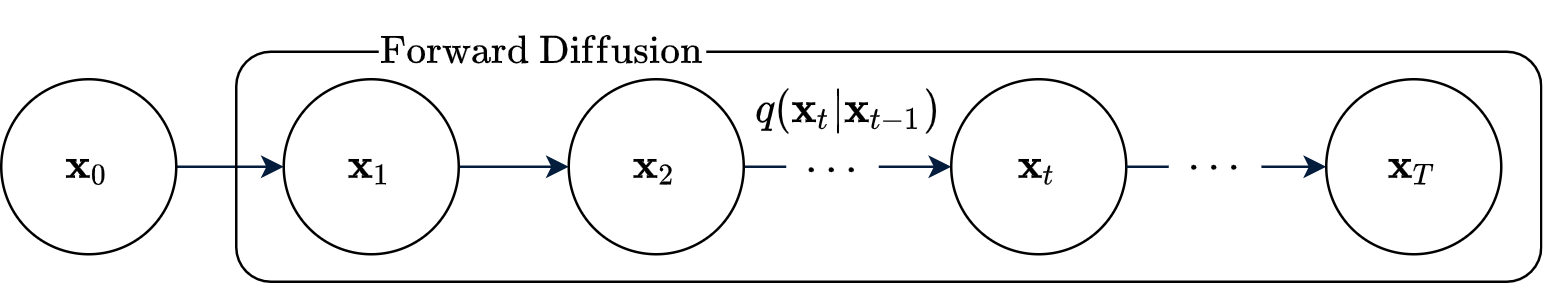
\includegraphics[width=0.8\linewidth]{figs/diffusion_pgm_forward}
    \end{figure}
    \eqpause
    \vspace{-0.3cm}
    \begin{block}{Forward Diffusion}
        \begin{itemize}
            \item Variational posterior distribution (encoder)
            \vspace{-0.3cm}
            \[
                q(\bz | \bx) = q(\bx_1, \dots, \bx_T | \bx_0) = \prod_{t = 1}^T q(\bx_t | \bx_{t - 1}).
            \]
            \item \textbf{Note:} there are no learnable parameters.
        \end{itemize}
        \vspace{-0.5cm}
    \end{block}
\end{frame}
%=======
\begin{frame}{Gaussian Diffusion Model as VAE}
    \myfootnotewithlink{https://ayandas.me/blog-tut/2021/12/04/diffusion-prob-models.html}{Das A. An Introduction to Diffusion Probabilistic Models, blog post, 2021}
    \[
        \pt(\bx, \bz) = \pt(\bx | \bz) \pt(\bz)
    \]    
    \eqpause
    \vspace{-0.5cm}
    \begin{figure}
        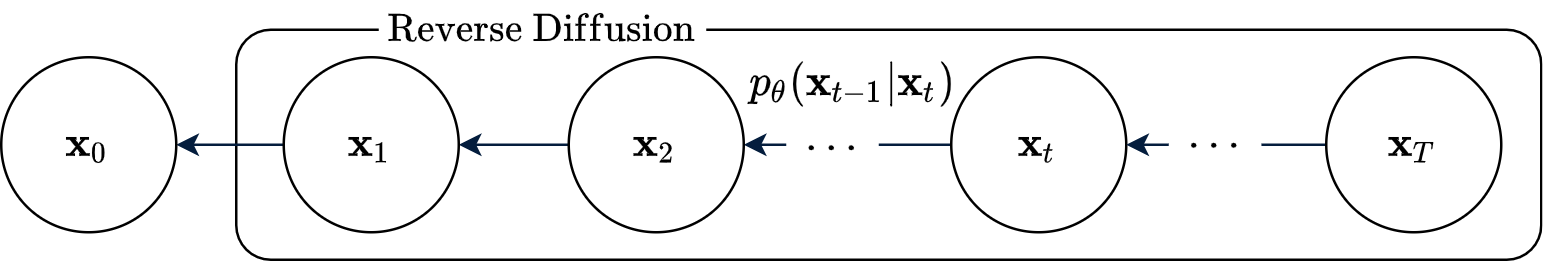
\includegraphics[width=0.8\linewidth]{figs/diffusion_pgm_reverse}
    \end{figure}
    \eqpause
    \vspace{-0.2cm}
    \begin{block}{Reverse Diffusion}
        \begin{itemize}
            \item Generative distribution (decoder)
            \[
                \pt(\bx | \bz) = \pt(\bx_0 | \bx_1).
            \]
            \vspace{-0.7cm}
            \eqpause
            \item Prior distribution
            \vspace{-0.3cm}
            \[
                \pt(\bz) = \pt(\bx_1, \dots, \bx_T) = \prod_{t=2}^T \pt(\bx_{t - 1} | \bx_t)  \cdot p(\bx_T).
            \]
            \vspace{-0.3cm}
        \end{itemize}
        \eqpause
        \textbf{Note:} This differs from the vanilla VAE due to the simple decoder $\pt(\bx | \bz)$ and the complex prior $\pt(\bz)$ (Markov chain).
    \end{block}
\end{frame}
%=======
\section{Diffusion ELBO Derivation}
%=======
\begin{frame}{ELBO for Gaussian Diffusion Model}
    \myfootnotewithlink{https://arxiv.org/abs/2006.11239}{Ho J. Denoising Diffusion Probabilistic Models, 2020}
    \begin{block}{Standard ELBO}
        \vspace{-0.3cm}
        \[
            \log \pt(\bx) \geq \bbE_{q({\color{teal}\bz} | \bx)} \log \frac{\pt(\bx, {\color{teal}\bz})}{q({\color{teal}\bz} | \bx)} = \cL_{\bphi, \btheta}(\bx) \rightarrow \max_{\bphi, \btheta}
        \]
        \vspace{-0.5cm}
    \end{block}
    \eqpause
    \begin{block}{Derivation}
        \vspace{-0.5cm}
        \begin{align*}
            \cL_{\bphi, \btheta}(\bx) &= \bbE_{q({\color{teal}\bx_{1:T}} | \bx_0)} \log \frac{\pt(\bx_0, {\color{teal}\bx_{1:T}})}{q({\color{teal}\bx_{1:T}} | \bx_0)} \\
            \nextonslide{& = \bbE_{q(\bx_{1:T} | \bx_0)} \log \frac{p(\bx_T) \prod_{t=1}^T \pt(\bx_{t-1} | \bx_t) }{\prod_{t=1}^T {\color{violet}q(\bx_t | \bx_{t-1})}}}
        \end{align*}
        \vspace{-0.3cm}
        \eqpause
        \begin{itemize}
            \item Let's try to decompose the ELBO into individual KL divergence terms.
            \item We need to replace $q(\bx_t | \bx_{t - 1})$ with $q(\bx_{t - 1} | \bx_t)$ in the denominator.
            \item Let's condition on $\bx_0$ to make the reverse $q(\bx_{t - 1} | \bx_t)$ tractable.
        \end{itemize}
    \end{block}
\end{frame}
%=======
\begin{frame}{ELBO for Gaussian Diffusion Model}
    \myfootnotewithlink{https://arxiv.org/abs/2006.11239}{Ho J. Denoising Diffusion Probabilistic Models, 2020}
    \[
         {\color{teal}q(\bx_t | \bx_{t-1}, \bx_0)}  = \frac{q(\bx_{t-1}|\bx_t, \bx_0)q(\bx_{t} | \bx_0)}{q(\bx_{t-1}| \bx_0)}
    \]
    \eqpause
    \vspace{-0.3cm}
    \begin{block}{Derivation (continued)}
        \vspace{-0.6cm}
        {\small
        \begin{align*}
            \cL_{\bphi, \btheta}(\bx) & = \bbE_{q(\bx_{1:T} | \bx_0)} \log \frac{p(\bx_T) \prod_{t=1}^T \pt(\bx_{t-1} | \bx_t) }{\prod_{t=1}^T {\color{violet}q(\bx_t | \bx_{t-1})}}  \\ 
            \nextonslide{& = \bbE_{q(\bx_{1:T} | \bx_0)} \log \frac{p(\bx_T) \prod_{t=1}^T \pt(\bx_{t-1} | \bx_t) }{\prod_{t=1}^T q(\bx_t | \bx_{t-1}, {\color{olive}\bx_0})}  }\\ 
            \nextonslide{& = \bbE_{q(\bx_{1:T} | \bx_0)} \log \frac{p(\bx_T) \pt(\bx_0 | \bx_1) \prod_{t=2}^T \pt(\bx_{t-1} | \bx_t) }{q(\bx_1 | \bx_0)\prod_{t=2}^T {\color{teal}q(\bx_t | \bx_{t-1}, \bx_0)}} }\\
            \nextonslide{& = \bbE_{q(\bx_{1:T} | \bx_0)} \log \frac{p(\bx_T) \pt(\bx_0 | \bx_1) \prod_{t=2}^T \pt(\bx_{t-1} | \bx_t) }{{\color{violet}q(\bx_1 | \bx_0)}\prod_{t=2}^T \frac{q(\bx_{t-1}|\bx_t, \bx_0) {\color{violet}q(\bx_{t} | \bx_0)}}{{\color{violet}q(\bx_{t-1}| \bx_0)}}} }\\
            \nextonslide{& = \bbE_{q(\bx_{1:T} | \bx_0)} \log \frac{{\color{violet}p(\bx_T)} {\color{olive}\pt(\bx_0 | \bx_1)} \prod_{t=2}^T \pt(\bx_{t-1} | \bx_t) }{{\color{violet}q(\bx_T | \bx_0)}\prod_{t=2}^T q(\bx_{t-1}|\bx_t, \bx_0)} }
        \end{align*}}
    \end{block}
\end{frame}
%=======
\begin{frame}{ELBO for Gaussian Diffusion Model}
    \myfootnotewithlink{https://arxiv.org/abs/2006.11239}{Ho J. Denoising Diffusion Probabilistic Models, 2020}
    \begin{block}{Derivation (continued)}
        \vspace{-0.7cm}
        {\small
        \begin{multline*}
            \cL_{\bphi, \btheta}(\bx) = \bbE_{q(\bx_{1:T} | \bx_0)} \log \frac{{\color{violet}p(\bx_T)} {\color{olive}\pt(\bx_0 | \bx_1)} \prod_{t=2}^T \pt(\bx_{t-1} | \bx_t) }{{\color{violet}q(\bx_T | \bx_0)}\prod_{t=2}^T q(\bx_{t-1}|\bx_t, \bx_0)} 
            \nextonslide{ = \\ = \bbE_{{\color{teal}q(\bx_{1:T} | \bx_0)}} \biggl[ \log {\color{olive}\pt(\bx_0 | \bx_1)} + \log {\color{violet}\frac{p(\bx_T)}{q(\bx_T | \bx_0)}} + \sum_{t=2}^T \log \left( \frac{\pt(\bx_{t-1} | \bx_t)}{q(\bx_{t-1}|\bx_{t}, \bx_0)}\right) \biggr] }
            \nextonslide{= \\ = \bbE_{{\color{teal}q(\bx_1 | \bx_0)}} \log \pt(\bx_0 | \bx_1) + \bbE_{{\color{teal}q(\bx_T | \bx_0)}} \log \frac{p(\bx_T)}{q(\bx_T | \bx_0)} + \\
             + \sum_{t=2}^T \bbE_{{\color{teal}q(\bx_{t-1}, \bx_t | \bx_0)}} \log \left( \frac{\pt(\bx_{t-1} | \bx_t)}{q(\bx_{t-1}|\bx_{t}, \bx_0)}\right) }
            \nextonslide{= \\ = \bbE_{q(\bx_1 | \bx_0)} \log \pt(\bx_0 | \bx_1) - \KL\bigl(q(\bx_T | \bx_0) \| p(\bx_T)\bigr) - \\
            - \sum_{t=2}^T \underbrace{ \bbE_{q(\bx_t | \bx_0)} \KL \bigl(q(\bx_{t-1} | \bx_t, \bx_0) \| \pt(\bx_{t-1} | \bx_t)\bigr)}_{\cL_t}}
        \end{multline*}
        }
        \vspace{-0.3cm}
    \end{block}
\end{frame}
%=======
\begin{frame}{ELBO for Gaussian Diffusion Model}
    \myfootnotewithlink{https://arxiv.org/abs/2006.11239}{Ho J. Denoising Diffusion Probabilistic Models, 2020}
        \vspace{-0.5cm}
        \begin{multline*}
            \cL_{\bphi, \btheta}(\bx) =  {\color{olive}\bbE_{q(\bx_1 | \bx_0)} \log \pt(\bx_0 | \bx_1)} - {\color{violet}\KL\bigl(q(\bx_T | \bx_0) \| p(\bx_T)\bigr)} - \\
            - {\color{teal}\sum_{t=2}^T \underbrace{ \bbE_{q(\bx_t | \bx_0)} \KL \bigl(q(\bx_{t-1} | \bx_t, \bx_0) \| \pt(\bx_{t-1} | \bx_t)\bigr)}_{\cL_t}}
        \end{multline*}
        \vspace{-0.5cm}
    \eqpause
    \begin{itemize}
        \item {\color{olive}First term} is the decoder distribution
        \[
            \log \pt(\bx_0 | \bx_1) = \log \cN \bigl(\bx_0 | \bmu_{\btheta, 1}(\bx_1), \bsigma_{\btheta, 1}^2(\bx_1)\bigr),
        \] 
        with $\bx_1 \sim q(\bx_1 | \bx_0)$.
        \eqpause
        \item {\color{violet}Second term} is constant: 
        \begin{itemize}
            \item $p(\bx_T) = \cN(0, \bI)$;
            \item $q(\bx_T | \bx_0) = \cN(\sqrt{\bar{\alpha}_T} \cdot \bx_0, (1 - \bar{\alpha}_T) \cdot \bI)$.
        \end{itemize}
        \eqpause
        \item {\color{teal}Third term} is the main contributor to the ELBO.
    \end{itemize}
\end{frame}
%=======
\begin{frame}{Summary}
	\begin{itemize}
		\item The Gaussian diffusion process is a Markov chain that incrementally corrupts data with specific Gaussian noise.
		\vfill
		\item Denoising score matching, together with Langevin dynamics, can be applied to the Gaussian diffusion process.
		\vfill
		\item The reverse process reconstructs data from noise samples, although its precise form is intractable.
        \vfill 
        \item We approximate the reverse process using normality assumptions.     
        \vfill
        \item Gaussian diffusion model can be interpreted as a VAE with a hierarchy of latent variables.
        \vfill
        \item The ELBO for Gaussian diffusion model may be formulated as a sum over many KL divergence terms.
	\end{itemize}
\end{frame}
%=======
\end{document}